~\label{chap:moseg}
\begin{chapterabstract}
This chapter introduces an approach to motion segmentation and dense reconstruction 
in dynamic scenes with RGBD observations. The approach outlined in this chapter is 
capable of performing dense reconstruction in dynamic environments and segmenting objects 
undergoing motion. The approach presented in this chapter yields an improvement in pose 
estimation accuracy with respect to the standard KinectFusion-like pipeline. Furthermore, 
it is demonstrated that the segmentation of dynamic objects may be leveraged for semantic 
purposes.
\end{chapterabstract}

\section{Introduction}
~\label{sec:moseg_introduction}
Progress in dense volumetric fusion has been accelerated in recent years with
the availability of consumer grade RGBD sensors such as the Microsoft Kinect and
the Asus Xtion coupled with the increasingly parallel nature of GPU hardware. Systems such 
as the seminal KinectFusion~\cite{Newcombe2011} allow one to build high quality, globally 
consistent scene models trivially, as outlined in Section~\ref{sec:intro_scene_recon} and 
Figure~\ref{figure:room_recon_example}.
Applications of such reconstruction pipelines however are limited due to the 
inability of such systems to handle scenes in which there are dynamics; these 
systems are unable to yield reliable reconstructions when there is motion in the 
sensors field of view, independent of the sensors own motion. Such a scenario introduces
additional error to the pose estimation component of the pipeline, resulting in
model corruption ranging from noise in the reconstruction to spurious 
surface data due to erroneous pose estimation.

In this chapter, an approach to mitigating the problems present when performing 
dense volumetric reconstruction in dynamic scenes is presented. The basic SLAM 
pipeline on which this work is based is the \textit{InfiniTAM}~\cite{Prisacariu2014} 
variant of the \textit{KinectFusion}~\cite{Newcombe2011} pipeline (InfiniTAM is also used 
as a base of comparison in Section~\ref{sec:moseg_quantitative}). Central to the
proposed, modified pipeline is the introduction of a dual scene representation based on 
the use of an implicit TSDF~\cite{Curless1996}. The use of a dual TSDF approach allows
for the segmentation of moving components in the scene from static components,
e.g.\ segmenting a person getting up from a chair from the chair itself. One of
the two scene representations is the \textit{static} scene and the other the
\textit{dynamic} scene. Such separation prevents corruption in the static scene,
the reconstruction output of the system. Examples of motion segmentation are given in 
Figure~\ref{figure:moseg_teaser}.
\begin{figure}[!htbp]
	\centering
	\begin{tabular}{ccc}
    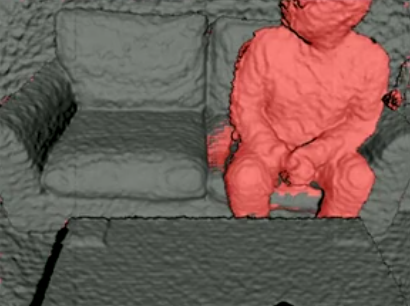
\includegraphics[width=.3\linewidth]{figures/moseg/teaser/sitting.png}&
    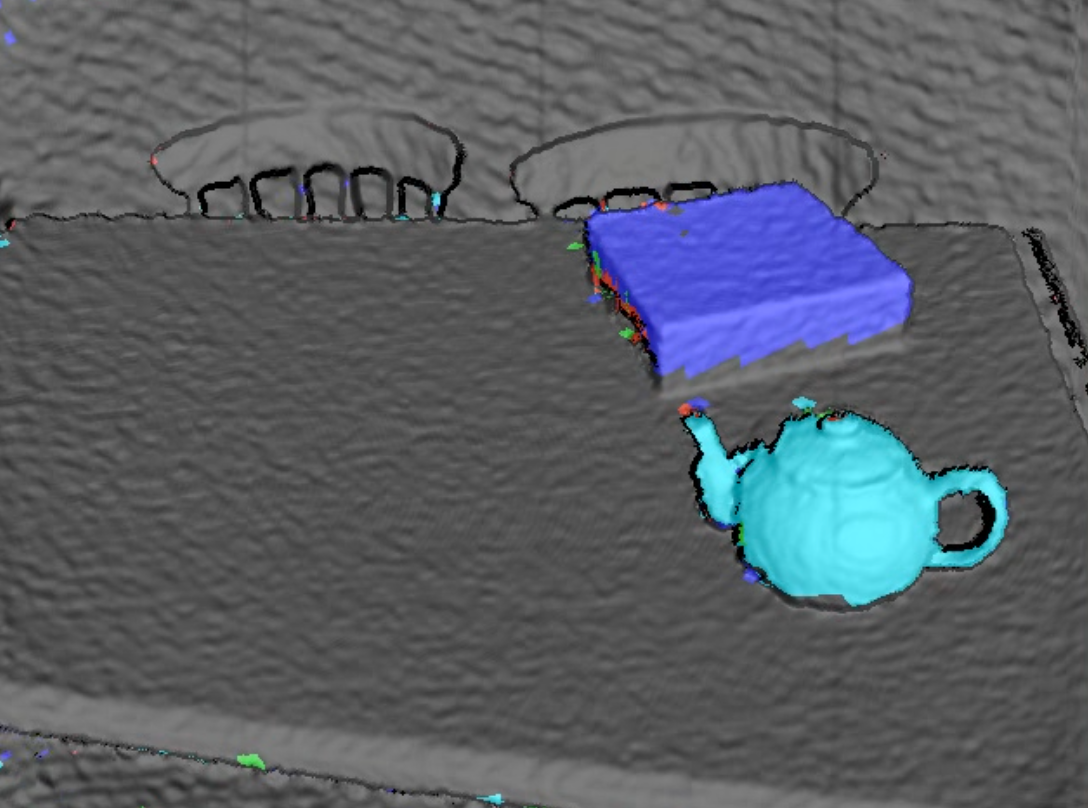
\includegraphics[width=.3\linewidth]{figures/moseg/teaser/objects.png}&
    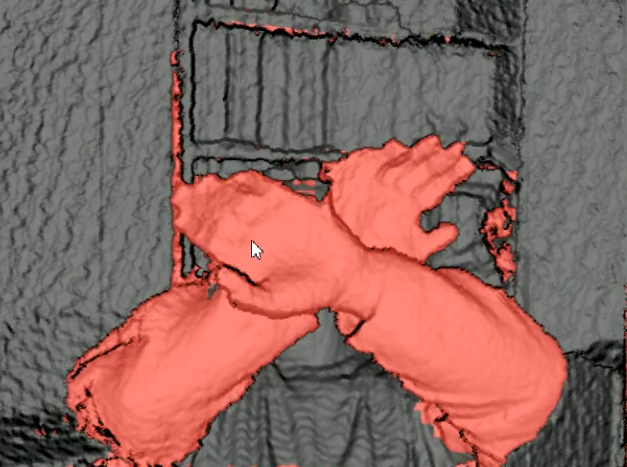
\includegraphics[width=.3\linewidth]{figures/moseg/teaser/arms.png}\\
    (a) & (b) & (c)\\
	\end{tabular}
  \caption[Motion Segmentation Example]
  {
    \begin{tabular}[t]{@{}l@{}}
      Examples of motion segmentation (note that red indicates motion):\\
      (a) A person sits on a setee.\\
      (b) Dynamic objects that have become stable and semantically identified.\\
      (c) A person waving their arms in the scene.
    \end{tabular}
  }
~\label{figure:moseg_teaser}
\end{figure}

Without the segmentation of dynamic scene components, when tracking against the
current reconstruction the integrated dynamic components may cause artefacts
that prevent the finding of ICP correspondences which often causes camera
tracking to drift, or completely fail. By tracking against only the stable
scene components, this interference in the ICP pose estimation process can be
mitigated.

% TODO: Chack spacing, which changes from this point.
Once a part of the dynamic model has been stable for a sufficient period, its
volumetric data is integrated in to the static model and is used for the
tracking phase of the pipeline. The use of volumetric structures in this work
is motivated by previous works on Voxel Block Hashing~\cite{NieBner2013},
providing efficient, real time lookup operations. The presented approach
exploits the abstraction that voxel blocks provide; a block of voxels is
interpreted as a region of space that can be either static or dynamic.
Voxel block stability is determined by a confidence measure over the voxel
blocks in the dynamic scene, such that isosurface information is not transferred
to the static model (used for camera tracking) until there is sufficient
confidence in it's stability. From a survey of the literature, it appears that 
this approach is the first to utilise such a dual representation for the motion 
segmentation problem. A graphical representation of the voxel block based structure 
of a given scene is presented in Figure~\ref{figure:voxel_blocks}.
% Based on http://www.texample.net/tikz/examples/sudoku-3d-cube/.
\begin{figure}[!htbp]
  \centering
  \resizebox{.6\linewidth}{!}{
    \begin{tikzpicture}[every node/.style={minimum size=1cm},on grid]
      %%%%%%%%%%%%%%%%%%%%%%%%%%%%%%%%%%%%%%%%%%%%%%%%%%%%%%%%%%%%%%%%%%%%%%%%%%
      %%% BEGIN: BIG GRID.
      %%%%%%%%%%%%%%%%%%%%%%%%%%%%%%%%%%%%%%%%%%%%%%%%%%%%%%%%%%%%%%%%%%%%%%%%%%
      % Left face nodes.
      \begin{scope}[every node/.append style={yslant=-0.5},yslant=-0.5]
        \foreach \i in {0,...,4}{
          \foreach \j in {0,...,4}{
            \ifthenelse{\i=4 \AND \j=4}{
              \node[fill=red!20] at (\i+0.5, \j+0.5) {vb};
            }{
              \node[fill=blue!20] at (\i+0.5, \j+0.5) {vb};
            }
          }
        }
        \draw (0,0) grid (5,5);
      \end{scope}

      % Right face nodes.
      \begin{scope}[every node/.append style={yslant=0.5},yslant=0.5]
        \foreach \i in {0,...,4}{
          \foreach \j in {0,...,4}{
            \ifthenelse{\i=0 \AND \j=0}{
              \node[fill=red!20] at (\i+5.5, -1*\j-0.5) {vb};
            }{
              \node[fill=blue!20] at (\i+5.5, -1*\j-0.5) {vb};
            }
          }
        }
        \draw(5, -5) grid (10, 0);
      \end{scope}

      % Top face nodes.
      \begin{scope}[every node/.append style={yslant=0.5,xslant=-1},yslant=0.5,xslant=-1]
        \foreach \i in {0,...,4}{
          \foreach \j in {4,...,0}{
            \ifthenelse{\i=0 \AND \j=0}{
              \node[fill=red!20] at (\i+5.5, \j+0.5) {\rotatebox{-45}{vb}};
            }{
              \node[fill=blue!20] at (\i+5.5, \j+0.5) {\rotatebox{-45}{vb}};
            }
          }
        }
        \draw (5,0) grid (10,5);
      \end{scope}
      \node at (5,-4) {\huge \textbf{Voxel Block Volume}};
      %%%%%%%%%%%%%%%%%%%%%%%%%%%%%%%%%%%%%%%%%%%%%%%%%%%%%%%%%%%%%%%%%%%%%%%%%%
      %%% END: BIG GRID.
      %%%%%%%%%%%%%%%%%%%%%%%%%%%%%%%%%%%%%%%%%%%%%%%%%%%%%%%%%%%%%%%%%%%%%%%%%%

      %%%%%%%%%%%%%%%%%%%%%%%%%%%%%%%%%%%%%%%%%%%%%%%%%%%%%%%%%%%%%%%%%%%%%%%%%%
      %%% BEGIN: SMALL GRID.
      %%%%%%%%%%%%%%%%%%%%%%%%%%%%%%%%%%%%%%%%%%%%%%%%%%%%%%%%%%%%%%%%%%%%%%%%%%
      \begin{scope}[shift={(14,-1)}]
        % Left face nodes.
        \begin{scope}[every node/.append style={yslant=-0.5},yslant=-0.5]
          \foreach \i in {0,...,2}{
            \foreach \j in {0,...,2}{
              \node[fill=red!20] at (\i+0.5, \j+0.5) {v};
            }
          }
          \draw (0,0) grid (3,3);
        \end{scope}

        % Right face nodes.
        \begin{scope}[every node/.append style={yslant=0.5},yslant=0.5]
          \foreach \i in {0,...,2}{
            \foreach \j in {0,...,2}{
              \node[fill=red!20] at (\i+3.5, -1*\j-0.5) {v};
            }
          }
          \draw(3, -3) grid (6, 0);
        \end{scope}

        % Top face nodes.
        \begin{scope}[every node/.append style={yslant=0.5,xslant=-1},yslant=0.5,xslant=-1]
          \foreach \i in {0,...,2}{
            \foreach \j in {2,...,0}{
              \node[fill=red!20] at (\i+3.5, \j+0.5) {\rotatebox{-45}{v}};
            }
          }
          \draw (3,0) grid (6,3);
        \end{scope}
        \node at (3,-3) {\huge \textbf{Voxel Volume}};
      \end{scope}
      %%%%%%%%%%%%%%%%%%%%%%%%%%%%%%%%%%%%%%%%%%%%%%%%%%%%%%%%%%%%%%%%%%%%%%%%%%
      %%% END: SMALL GRID.
      %%%%%%%%%%%%%%%%%%%%%%%%%%%%%%%%%%%%%%%%%%%%%%%%%%%%%%%%%%%%%%%%%%%%%%%%%%
    \end{tikzpicture}
  }
  \caption[TSDF split in to voxel blocks]{A graphical representation of an 
  SDF/TSDF with it's voxels subdivided into voxel blocks. In the above, \(v\) 
  represents voxel blocks and \(v\) voxels.}
~\label{figure:voxel_blocks}
\end{figure}

The remainder of this chapter is structured as follows.
Section~\ref{sec:moseg_static_fusion} introduces preliminaries pertaining to 
the static Fusion pipeline followed by Section~\ref{sec:moseg_dynamic_fusion} 
describing the dynamic Fusion component of theipeline. Qualitative and quantitative 
results are presented in Sections~\ref{sec:moseg_qualitative} and~\ref{sec:moseg_quantitative}, 
respectively. Finally, an application to interactive object recognition is given in Section
~\ref{sec:moseg_semantic}.

\section{Static Volumetric Fusion}
~\label{sec:moseg_static_fusion}
The volumetric fusion approach taken in this work draws on previous volumetric
integration techniques~\cite{Curless1996, Newcombe2011, NieBner2013, Prisacariu2014} 
and shall be introduced in this section as preliminary material as it shall be
referred to in later chapters. Following this approach, at each frame the camera
is tracked against the current scene, after which new data is fused into the
scene model which is then rendered using raycasting to prepare for tracking in
the next frame.

The static Fusion pipeline consists of the following three consecutive steps:
\begin{itemize}
  \item Camera Tracking.
  \item Model Integration.
  \item Rendering.
\end{itemize}

The approach in this work utilises the TSDF Volumetric data structure which
encodes for each voxel in the structure, a signed value and a weight.
In the case of 3D environment modelling, the values pertain to distances from
surfaces, within some truncation region.

Given a vertex map generated from the back projection of the points in a depth
image, the vertices pertain to the zero crossing point with voxels either side
representing distances to the zero crossing point; positive in front of the
surface, negative behind. Surface points are known as the Zero Level Set.
\begin{figure}[!htbp]
  \centering
  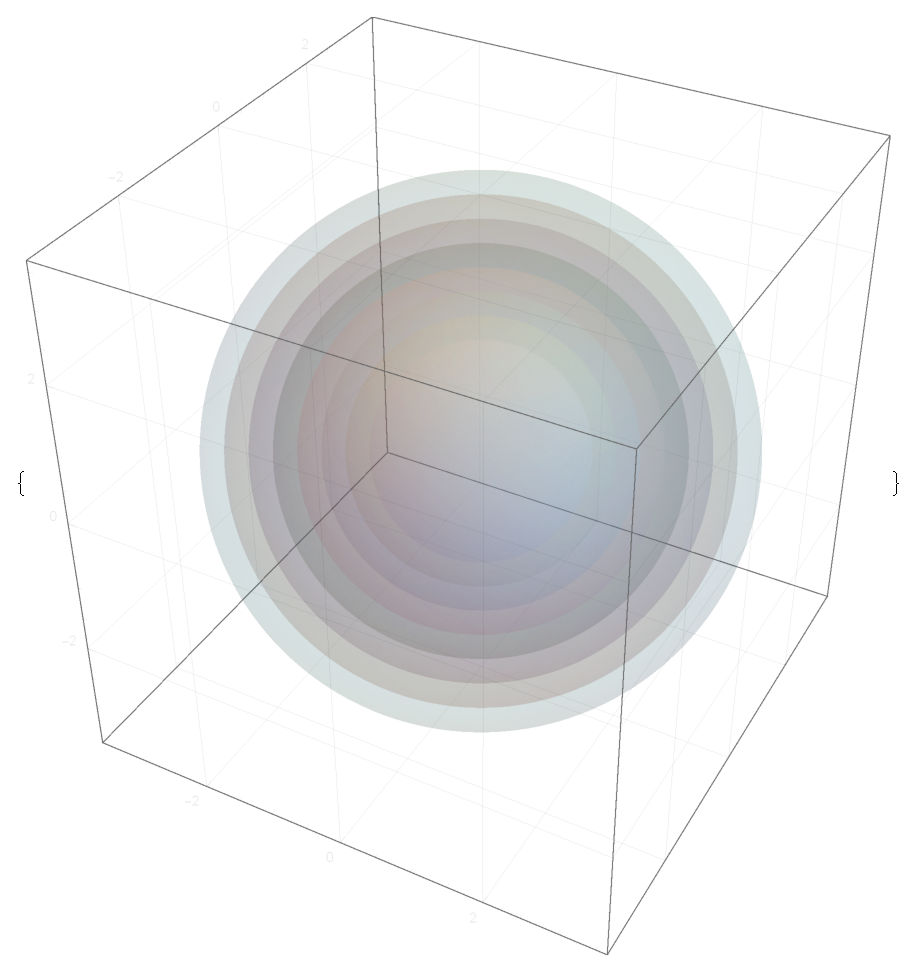
\includegraphics[width=.6\linewidth]{figures/moseg/3d_sdf.eps}
  \caption[Signed Distance Function]{An example of a sphere embedded within a 
  three dimensional SDF.}
~\label{figure:sdf_example}
\end{figure}

For a given TSDF \(\bm{\Phi}\), the Zero Level Set is defined as follows in Equation
~\ref{eqn:zeri_level_definition} where \(v\) denotes a TSDF voxel. An example of such an 
embedding is given in Figure~\ref{figure:sdf_example}.
\begin{equation}
  \label{eqn:zero_level_definition}
  \mathcal{S} = \{v \given \bm{\Phi}(v) = 0\}, 
  \mkern2mu \forall \mkern2mu v \in \bm{\Phi}
\end{equation}

To facilitate real time fusion, the InfiniTAM framework employs a voxel block
hashing mechanism for fast access to scene voxels~\cite{NieBner2013}. Within
this context, voxel blocks are collections of \(\mathbb{R}^{N \times N \times N}\) 
TSDF voxels, stored in a hash table for fast access. As such, each hash table entry 
corresponds to a portion of a global voxel block array, pertaining to a region in the 
scene. This division of the scene into voxel blocks is used for the later process of 
determining and labelling dynamic regions in the scene.

\subsection{Camera Pose Estimation}
~\label{subsec:moseg_static_camera_tracking}
As in previous works~\cite{Newcombe2011, Prisacariu2014}, the gradient
optimisation based ICP algorithm is utilised to register consecutive images
to derive the camera pose at time \(t\) with respect to time \(t-1\), that is to
optimise for the rigid body transform \(\bm{T} \in \mathbb{SE}(3)\) of the
camera between the two frames using the Levenberg-Marquardt nonlinear least
squares method~\cite{NumericalRecipes}. The rendering stage of the pipeline
is used to generate the image from the TSDF at time \(t-1\) to which a new frame
at time \(t\) is registered.

The target transformation \(\bm{T} \in \mathbb{SE}(3)\) is a member of the
Special Euclidean Group
\begin{equation}
  \label{eqn:se3_definition}
  \mathbb{SE}(3) = \{\bm{R}, \bm{t} \given \bm{R} \in
  \mathbb{SO}(3), \bm{t} \in \mathbb{R}^{3}\}
\end{equation}
and has the following form
\begin{equation}
  \label{eqn:trans_mat_definition}
  \bm{T} =
  \begin{bmatrix}
    \bm{R} & \bm{t} \\
    \bm{0} & 1
  \end{bmatrix}
\end{equation}
where \(\mathbb{SO}(3)\) is the Special Orthogonal Group of Skew Symmetric
Rotation Matrices.

\subsubsection{Attitude Representation}
~\label{subsub:moseg_static_camera_attitude}
The rotation matrix component of the transformation \(\bm{T}\) is
generated by a Rodriguez parameterization~\cite{Shuster1993}, whereby the
\(\mathbb{SO}(3)\) rotation matrix \(\bm{R}\) is generated by three rotational
parameters, \( \alpha \), \( \beta \) and \( \gamma \). Each parameter represents a 
rotation around one of three principal axes, as shown in Figure~\ref{figure:euler_axes}.
\begin{figure}[!htbp]
  \centering
  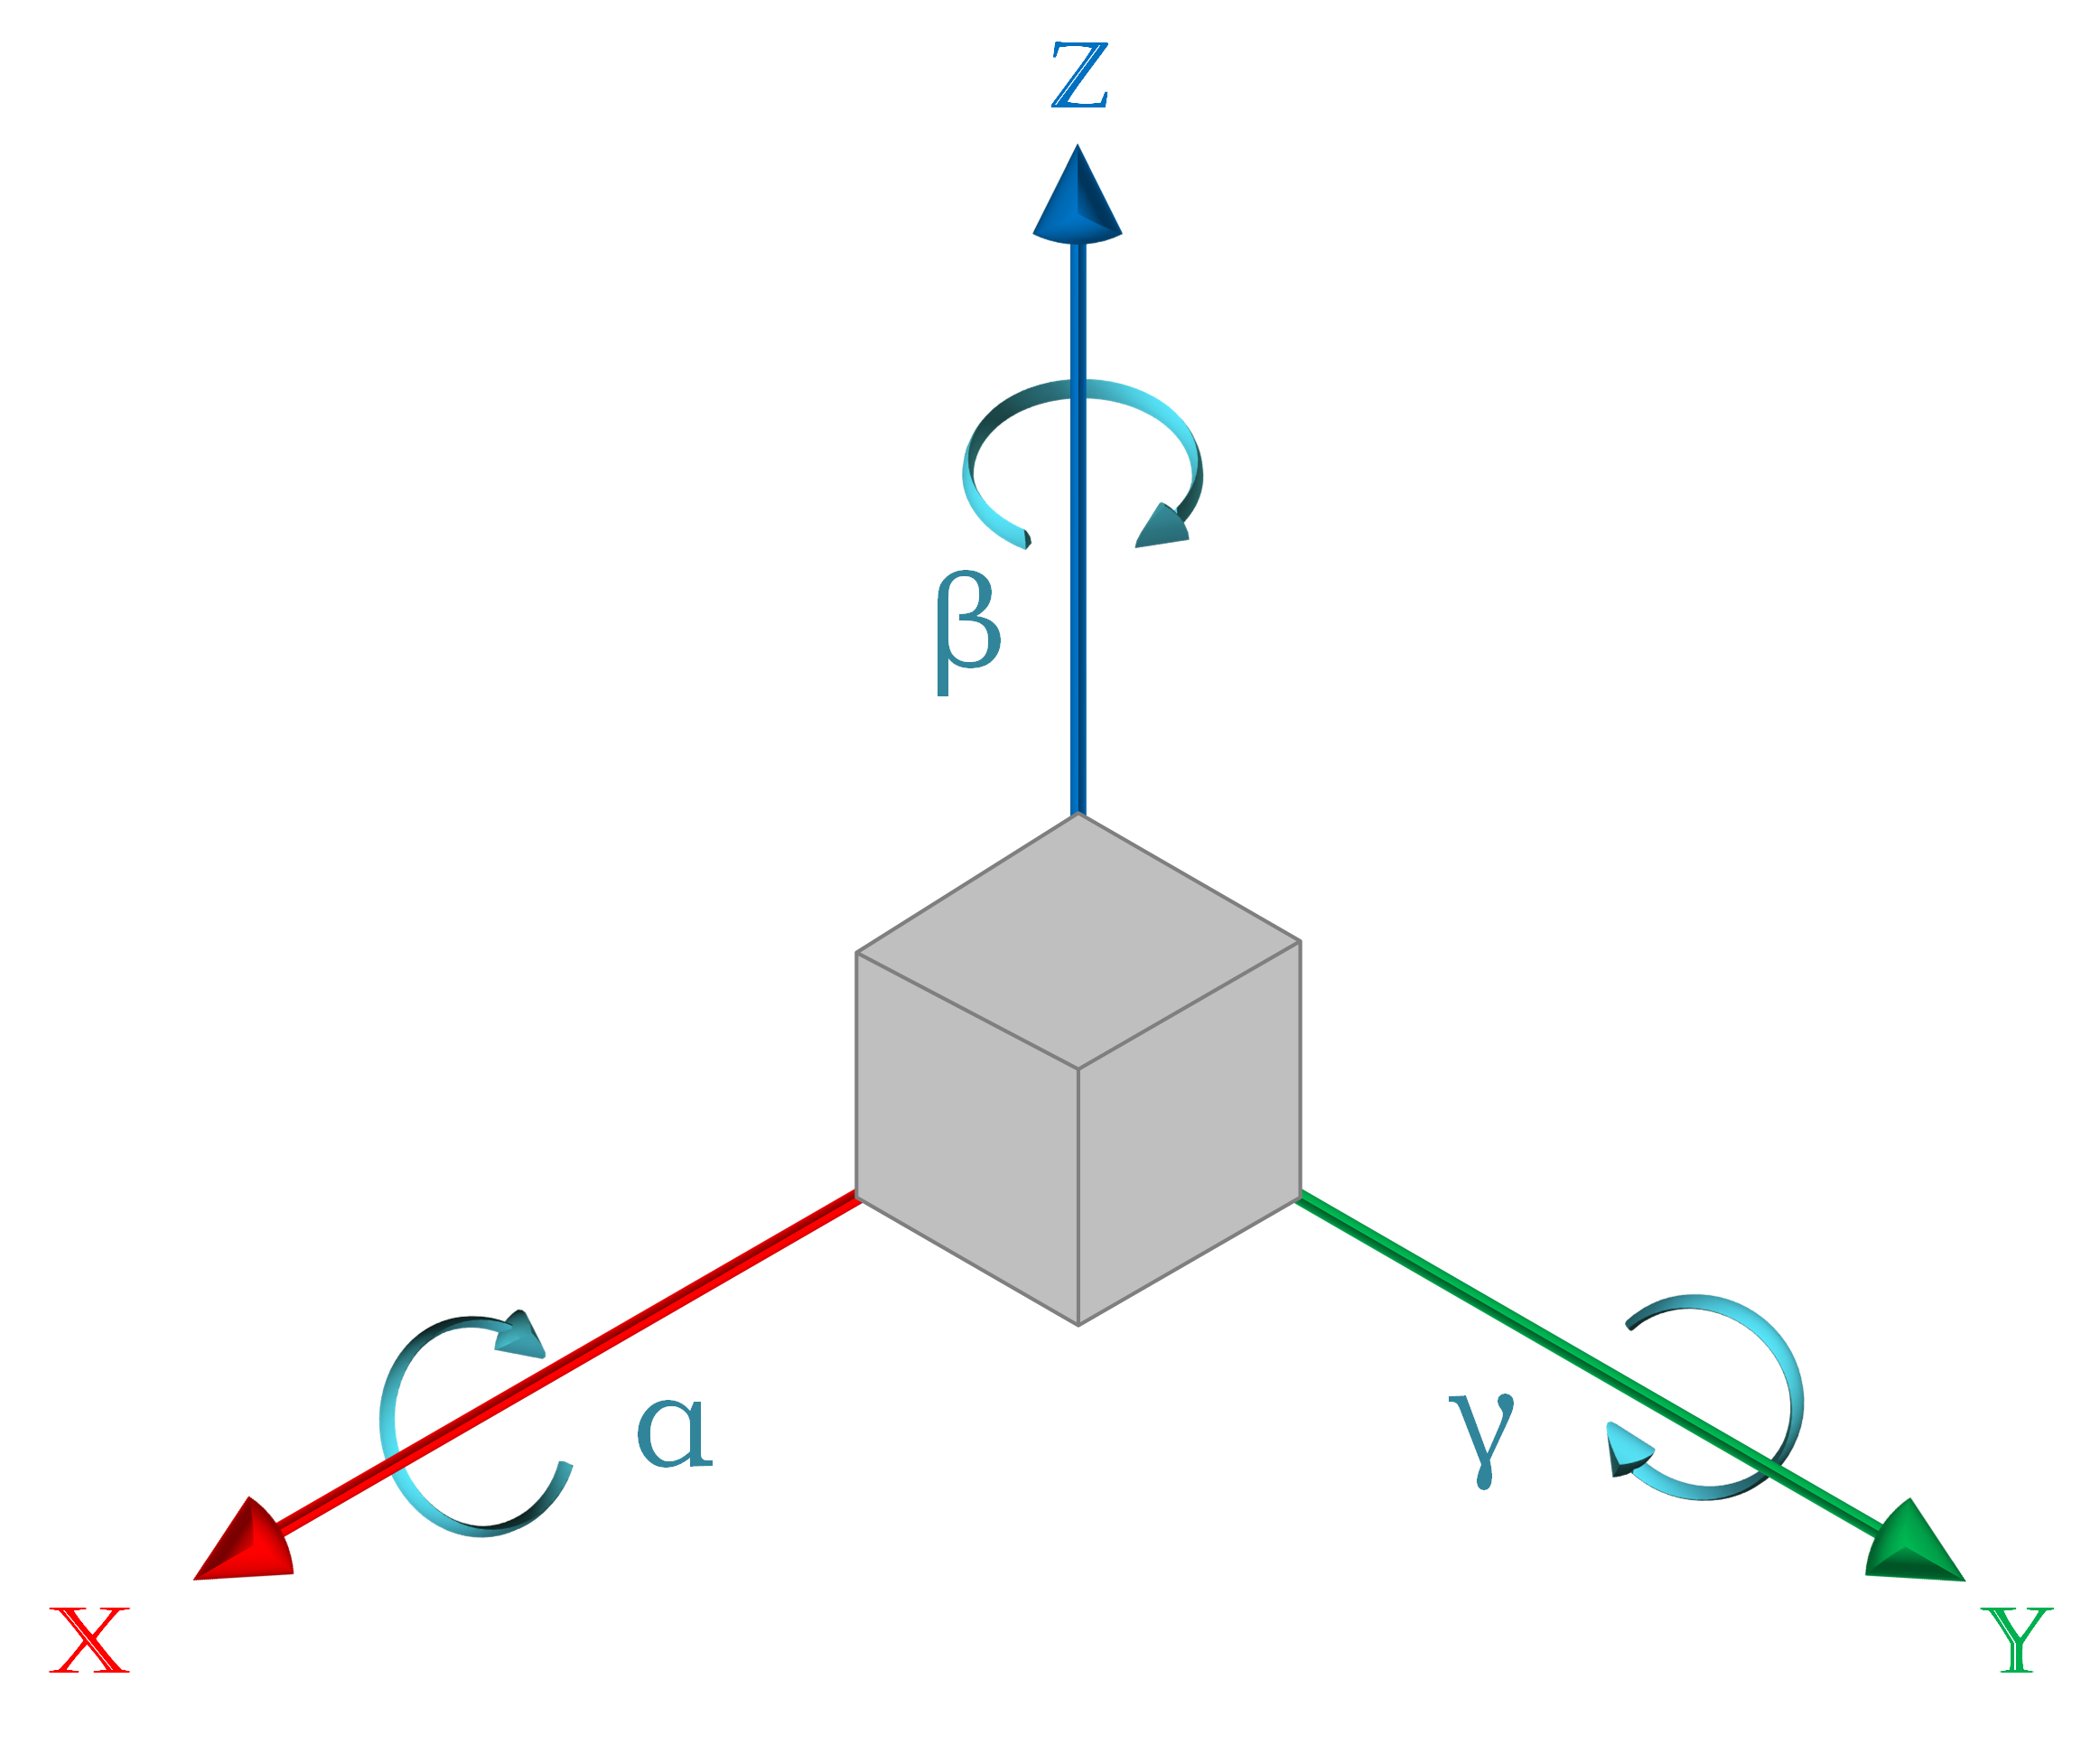
\includegraphics[width=.6\linewidth]{figures/moseg/euler_angles.png}
  \caption[Rotational Axes]{Right handed coordinate system and the three rotational axes; 
  \( \alpha \), \( \beta \) and \( \gamma \).}
~\label{figure:euler_axes}
\end{figure}

The Rodriguez parameters \( \alpha \), \( \beta \) and \( \gamma \) form a member of the Lie Algebra 
\( \mathfrak{g} \) corresponding to the tangent space of the \( \mathbb{SO}(3) \) Lie Group. Elements 
of the Lie Algebra map to the Lie Group by the matrix exponential.

The formulation of the Rodriguez parameterization (performing the aforementioned matrix exponential)
~\cite{Shuster1993} is given by Equation~\ref{eqn:rodriguez_matrix_eq}, with the parameter vector
\(\bm{p} = {[\alpha, \beta, \gamma]}^{T}\)
\begin{equation}
  \label{eqn:rodriguez_matrix_eq}
  \bm{R}(\bm{p}) =
  \frac{1}{\norm{\bm{p}}^{2}}
  \bigg[
  (1 - \norm{\bm{p}}^{2})\bm{I} +
  2 \bm{pp}^{T} + \omega(\bm{p})
  \bigg]
\end{equation}

Where for an arbitrary vector \(\bm{v}\), \(\omega(\bm{v})\) is defined as
the cross product matrix operator and is defined as follows in Equation~\ref{eqn:cross_prod_mat}.
% TODO: Tidy. Maybe merge into above equation?
\begin{equation}
  \label{eqn:cross_prod_mat}
  \omega(\bm{v}) =
  \begin{bmatrix}
    0 & v_{3} & -v_{2} \\
    -v_{3} & 0 & v_{1} \\
    v_{2} & -v_{1} & 0
  \end{bmatrix}
\end{equation}

Evaluating Equation~\ref{eqn:rodriguez_matrix_eq} leads to the following form
of the rotation matrix \(\bm{R}\)
\begin{equation}
  \label{eqn:rodriguez_matrix}
  \bm{R} = \frac{1}{\norm{\bm{p}}^{2} + 1}
  \begin{bmatrix}
    % Row 1.
    \alpha^{2} - \beta^{2} - \gamma^{2} + 1 &
    2 \alpha \beta + \gamma &
    2 \alpha \gamma - \beta \\
    % Row 2.
    2 \alpha \beta - \gamma &
    -(\alpha^{2} - \beta^{2} + \gamma^{2} - 1) &
    \alpha + 2 \beta \gamma \\
    % Row 3.
    2 \alpha \gamma + \beta &
    -(\alpha - 2 \beta \gamma) &
    -(\alpha^{2} + \beta^{2} - \gamma^{2} - 1)
  \end{bmatrix}
\end{equation}

The translational component \(\bm{t}\) of the transformation \(\bm{T}\) is
given by the following vector, with each component representing a translation
along it's respective axis.
\begin{equation}
  \label{eqn:trans_vector}
  \bm{t} =
  \begin{bmatrix}
    t_{x} \\
    t_{y} \\
    t_{z}
  \end{bmatrix}
\end{equation}

\subsubsection{Pose Recovery Formulation}
~\label{subsub:moseg_static_camera_poserec}
The recovery of the camera pose change between frames \(t\) and \(t-1\) may be
formulated as the following point-to-plane energy minimisation problem
\begin{equation}
  \label{eqn:pose_estimation_kf}
  E(\bm{R}, \bm{t}, \bm{\Omega}, \bm{\Phi}) =
  \argmin_{\bm{R}, \bm{t}} \sum_{p \in \bm{\Omega}}
  \norm{{\left[
    \bm{Rx} + \bm{t} - \mathcal{V}(\bar{\bm{x}})
  \right]}^{T}
  \mathcal{N}(\bar{\bm{x}})}
\end{equation}
where in Equation~\ref{eqn:pose_estimation_kf} \(\bm{R}\) and \(\bm{t}\) are 
the aforementioned rotation matrix and translation vector of the transformation 
\(\bm{T}\). \(\bm{x}\) is the 3D point extracted from the depth image 
\(\bm{\Omega}\) and the point \(\bar{\bm{x}}\) is the 3D point in the TSDF 
volume \(\bm{\Phi}\) found by raycasting from \(\bm{\Omega}\) under the 
transformation \(\bm{T}\). Finally, \(\mathcal{N}\) is a normal map of 
\(\bm{\Phi}\) and is defined as follows
\begin{equation}
  \label{eqn:normal_map_definition}
  \mathcal{N} = \frac{\nabla \bm{\Phi}}{\norm{\nabla \bm{\Phi}}}
\end{equation}
where \(\nabla \bm{\Phi}\) is approximated by central finite differencing, 
as follows in Equation~\ref{eqn:sdf_central_diff}.
\begin{equation}
  \label{eqn:sdf_central_diff}
  \nabla \bm{\Phi} = 
    \begin{bmatrix}
      {\big( 2 \delta \bm{v}_{x} \big)}^{-1} \\
      {\big( 2 \delta \bm{v}_{y} \big)}^{-1} \\
      {\big( 2 \delta \bm{v}_{z} \big)}^{-1}
    \end{bmatrix}
    \odot
    \begin{bmatrix}
      \bm{\Phi} \big(\bm{v}_{x} + \delta \bm{v}_{x}\big) - \bm{\Phi} \big(\bm{v}_{x} - \delta \bm{v}_{x}\big) \\
      \bm{\Phi} \big(\bm{v}_{y} + \delta \bm{v}_{y}\big) - \bm{\Phi} \big(\bm{v}_{y} - \delta \bm{v}_{y}\big) \\
      \bm{\Phi} \big(\bm{v}_{z} + \delta \bm{v}_{z}\big) - \bm{\Phi} \big(\bm{v}_{z} - \delta \bm{v}_{z}\big) 
    \end{bmatrix}
\end{equation}

For the gradient update phase of the ICP algorithm, the partial derivatives
\( \frac{\partial E}{\partial \bm{R}_{\lambda}} \forall \lambda \in \{\alpha, \beta, \gamma \} \) 
may be derived as follows in Equation~\ref{eqn:icp_update_derivation_rot}.
As a first step, the following definition is made
\begin{equation}
  \label{eqn:icp_deriv_sub}
  \phi(\bm{R}, \bm{t}, \bm{x}, \bar{\bm{x}}) =
  {\left[
    \bm{Rx} + \bm{t} - \mathcal{V}(\bar{\bm{x}})
  \right]}^{T}
  \mathcal{N}(\bar{\bm{x}})
\end{equation}
With this substitution in place, the derivation proceeds as follows
\begin{align}
  \label{eqn:icp_update_derivation_rot}
  % Line 1.
  \frac{\partial E}{\partial \lambda} ={}&
  \frac{\partial}{\partial \lambda}
  \sum_{p \in \bm{\Omega}}
  \norm{\phi(.)}\\
  % Line 2.
  ={}& \sum_{p \in \bm{\Omega}}
  \frac{\partial}{\partial \lambda}
  \norm{\phi(.)}\\
  % Line 3.
  ={}& \sum_{p \in \bm{\Omega}}
  \frac{\partial}{\partial \phi(.)} \norm{\phi(.)}
  \frac{\partial \phi(.)}{\partial \lambda}\\
  % Line 4.
  ={}& \sum_{p \in \bm{\Omega}}
  \frac{1}{2}{\frac{2 \phi(.)}{\sqrt{\phi(.)}^{T}\phi(.)}}
  \frac{\partial \phi(.)}{\partial \lambda}\\
  % Line 5.
  ={}& \sum_{p \in \bm{\Omega}}
  \frac{\phi(.)}{\norm{\phi(.)}}
  \frac{\partial \phi(.)}{\partial \lambda}\\
  % Line 6
  ={}& \sum_{p \in \bm{\Omega}}
  \frac{\phi(.)}{\norm{\phi(.)}}
  \Bigg[ \frac{\partial}{\partial \lambda}
  {\bigg[ \bm{Rx} + \bm{t} - \mathcal{V}(\bar{\bm{x}}) \bigg]}^{T}
  \mathcal{N}(\bar{\bm{x}}) + 
  {\bigg[ \bm{Rx} + \bm{t} - \mathcal{V}(\bar{\bm{x}}) \bigg]}^{T}
  \frac{\partial}{\partial \lambda}
  \mathcal{N}(\bar{\bm{x}})\Bigg]\\
  % Line 6
  ={}& \sum_{p \in \bm{\Omega}}
  \frac{\phi(.)}{\norm{\phi(.)}}
  {\bigg[ \frac{\partial \bm{R}}{\partial \lambda}
  \bm{x}\bigg]}^{T}
  \mathcal{N}(\bar{\bm{x}})
\end{align}
The full partial derivatives \(\frac{\partial \bm{R}}{\partial \alpha}\),
\(\frac{\partial \bm{R}}{\partial \beta}\) and
\(\frac{\partial \bm{R}}{\partial \gamma}\) may be found Equations
~\ref{eqn:rodrigues_full_alpha_deriv},~\ref{eqn:rodrigues_full_beta_deriv}
and~\ref{eqn:rodrigues_full_gamma_deriv} respectively, of Appendix 
~\ref{appendix:mathematical}.

The partial derivatives
\( \frac{\partial \bm{R}}{\partial \lambda} \forall \lambda \in \{\alpha, \beta, \gamma \} \) 
may be multiplied with \(\bm{x}\) and combined in to the following Rotation Jacobian
\begin{align}
  \label{eqn:rot_jac}
  \bm{J}_{R} ={}& \left. {\bigg[
    \frac{\partial \bm{R}}{\partial \lambda} \bm{x}
    \bigg]}^{T} \right\vert_{\lambda = 0} \\
  ={}&
  \begin{bmatrix}
    0 & -z & y \\
    z & 0 & -x \\
    -y & x & 0
  \end{bmatrix}
\end{align}

Note that the derivation for the partial derivatives
\(\frac{\partial E}{\partial \bm{t}_{\bar{\lambda}}} \forall \bar{\lambda} \in \{x, y, z\} \) 
is analogous with that of Equation~\ref{eqn:icp_update_derivation_rot}, with the result given as 
follows
\begin{equation}
  \label{eqn:icp_update_derivation_trans}
  \frac{\partial E}{\partial \bm{t}_{\bar{\lambda}}} =
  \sum_{p \in \bm{\Omega}}
  \frac{\phi(.)}{\norm{\phi(.)}}
  {\bigg[ \frac{\partial \bm{t}}{\partial \bar{\lambda}}\bigg]}^{T}
  \mathcal{N}(\bar{\bm{x}})
\end{equation}

The translational partial derivatives
\( \frac{\partial \bm{t}}{\partial \lambda} \forall \bar{\lambda} \in \{x, y, z\} \) may also 
be combined in to the following translation Jacobian as in Equation~\ref{eqn:rot_jac}.
\begin{equation}
  \label{eqn:trans_jac}
  \bm{J}_{t} =
  \begin{bmatrix}
    1 & 0 & 0 \\
    0 & 1 & 0 \\
    0 & 0 & 1
  \end{bmatrix}
\end{equation}

The overall combined Jacobian for the energy function defined in Equation
~\ref{eqn:pose_estimation_kf}, for use in pose optimisation is as follows
\begin{equation}
  \label{eqn:pose_jacobian}
  \bm{J} =
  \frac{\phi(.)}{\norm{\phi(.)}}
  \begin{bmatrix}
    \bm{J}_{R} & \bm{J}_{t}
  \end{bmatrix}^{T}
  \mathcal{N}(\bar{\bm{x}})
\end{equation}

\subsubsection{Pose Recovery Optimisation}
~\label{subsub:moseg_static_camera_poserec_opt}
With the gradient derivations in place, this section will now detail the
pose recovery procedure. As highlighted, the optimisation routine used is the
Levenberg-Marquardt~\cite{NumericalRecipes} algorithm for solving nonlinear least
squares problems. The gradient update equation for the Levenberg-Marquardt
algorithm is given as follows
\begin{equation}
  \label{eqn:lm_update}
  \theta_{t+1} = \theta_{t} - {(\bm{H} + \lambda \text{diag}(
  \bm{H}))}^{-1}
  \bm{J}
\end{equation}
where \(\theta_{t} = {[\alpha, \beta, \gamma, t_{x}, t_{y}, t_{z}]}^{T}\) is the
parameter vector of \(\bm{T}\) at time \(t\), \(\bm{J}\) is the Jacobian
introduced in Equation~\ref{eqn:pose_jacobian} and \(\bm{H}\) is the Hessian,
approximated by \(\bm{H} = \bm{J}^{T}\bm{J}\). The parameter \( \lambda \)
controls the influence of the gradient on the update step and is adjusted
according to the change in error, as shall be evident in the algorithm
that follows.

{
  \centering
  \singlespacing{}
  \begin{minipage}{.7\linewidth}
    \begin{algorithm}[H]
~\label{alg:icp}
      \caption{ICP with Levenberg-Marquardt}
      \begin{algorithmic}[1]
        % $.$ used instead of \(\) due to a bug(?) in algorithmic.
        \Procedure{ICP}{$\mathcal{D}_{l}, \mathcal{D}_{m}, \mathcal{V}, \theta_{t-1}$}
        \State{\( \lambda \gets \lambda_{init} \)}
        \State{\( \theta_{tmp} \gets \theta_{t-1} \)}
        \State{\( \theta_{t} \gets \theta_{tmp} \)}
        \State{\( \epsilon_{old} \gets \inf \)}
        \State{\( \epsilon \gets \epsilon_{old} \)}
        \While{\( \epsilon >= \tau \)}
        \State{\( \epsilon \gets E(.) \)}
        \Comment{Evaluate Equation~\ref{eqn:pose_estimation_kf}}
        \If{\( \epsilon \leq \epsilon_{old} \)}
        \State{\( \lambda \gets 10\lambda \)}
        \State{\( \theta_{t} \gets \theta_{tmp} \)}
        \Else{}
        \State{\( \lambda \gets \frac{\lambda}{10} \)}
        \State{\( \epsilon_{old} \gets \epsilon \)}
        \State{\( \theta_{tmp} \gets \theta_{t} \)}
        \EndIf{}
        \State{\( \bm{J} \gets \nabla E \)}
        \Comment{Evaluate Equation~\ref{eqn:pose_jacobian}}
        \State{\( \bm{H} = \bm{J}^{T}\bm{J} \)}
        \State{\( \bm{C} = \text{chol}(\bm{H} + \lambda \text{diag}(\bm{H})) \)}
        \State{\( \delta = \text{backsub}(\bm{C}, \bm{J}) \)}
        \State{\( \theta_{tmp} \gets \theta_{tmp} - \delta \)}
        \EndWhile{}
        \Return{\( \theta_{t} \)}
        \EndProcedure{}
      \end{algorithmic}
    \end{algorithm}
  \end{minipage}
  \par
}

Note that for numerical stability, the matrix inverse in Equation~\ref{eqn:lm_update} 
may be avoided by utilising the \texttt{chol} and \texttt{backsub} routines to 
compute the Cholesky Decomposition~\cite{NumericalRecipes} and solve a linear system with 
backsubstitution~\cite{ElemLinAlg}, respectively. Additionally, it should be noted that 
the cost term of Equation~\ref{eqn:pose_estimation_kf} and jacobian term of Equation
~\ref{eqn:pose_jacobian} may be evaluated and reduced on the GPU as there exists no spatial 
data dependence between either the model points or depth map points.

\subsection{Volumetric Integration}
~\label{subsec:moseg_static_integration}
The second phase in the scene reconstruction pipeline is volumetric integration.
That is, the integration of observed depth images into a consistent, implicit
volumetric representation, in this case the existing TSDF model of the scene,
providing the basis for an updated rendering to be used in the ICP procedure
for camera tracking at the next time step.

As previously outlined, the TSDF may be defined as a volume of distances to an
isosurface, with the isosurface itself being given by the Zero Level Set, as
defined in Equation~\ref{eqn:zero_level_definition}. A graphical representation
is given in Figure~\ref{figure:sdf_example}.

As with KinectFusion~\cite{Newcombe2011} the global (scene) location
\(\bm{x}_{v}\) of each voxel \(v \in \bm{\Phi}\) that is visible in the
current view frustum is transformed into the camera's coordinate frame via the
following transformation (noting that \(\bm{x}_{v}\) is in homogeneous form)
\begin{equation}
\label{eqn:project_tsdf_to_image}
\bm{x}_{\Omega} = \bm{K}\bm{T}_i^{-1}\bm{x}_{v}
\end{equation}
where \(\bm{K}\) is the camera's intrinsic calibration matrix, \(\bm{T}\) is
the transformation optimised for at time \(t\), with the form given in Equation
~\ref{eqn:trans_mat_definition} and \(\bm{x}_{\Omega}\) is the resultant
projected coordinates. The form of the camera intrinsic calibration is as 
follows.
\begin{equation}
  \label{eqn:camera_matrix}
  \bm{K} = 
  \begin{bmatrix}
    f_{x} & s & x_{0} & 0\\
    0 & f_{y} & y_{0} & 0\\
    0 & 0 & 1 & 0
  \end{bmatrix}
\end{equation}
Where in Equation~\ref{eqn:camera_matrix}, \(f_{x}\), \(f_{y}\), \(s\), \(x_{0}\) 
and \(y_{0}\) are the focal lengths, scale and camera principal points respectively.

The integration of new data points into the TSDF volume is achieved by computing 
running means; each voxel contains a running average of its SDF value over time.
Projecting to the depth image \(\bm{\Omega}\) coordinates as in Equation
~\ref{eqn:project_tsdf_to_image} to perform a depth pixel lookup in \(\bm{\Omega}\)
and subtracting the \(z\) component of \(\bm{x}_{v}\) from the resulting value
yields the depth offset from the surface, as follows
\begin{equation}
  \label{eqn:integration_offset}
  \eta = \bm{x}_{\Omega} - \bm{x}_{v}^{z}
\end{equation}

If \( \eta \geq -\mu \), that is that the depth of the point is not beyond the
truncation band of the TSDF behind the isosurface, where \( \mu \) is half the 
width of the truncation band, then the TSDF depth measurement update 
proceeds as follows for a voxel \(\bm{x}_{v} \in \bm{\Phi}\).
\begin{equation}
\label{eqn:sdf_update}
\bm{\Phi}{(\bm{x}_{v})}_{t} = \frac{1}{\phi{(\bm{x}_{v})}_{t-1} + 1}
\bigg[\phi{(\bm{x}_{v})}_{t-1}\bm{\bm{\Phi}}{(\bm{x}_{v})}_{t-1} +
\text{min} \bigg( 1, \frac{\eta}{\mu} \bigg)
\bigg]
\end{equation}

\begin{figure}[!htbp]
  \caption{TODO}
~\label{figure:truncation_band}
\end{figure}

In addition, the weight \(\phi(\bm{x}_{v})\) is updated as follows.
\begin{equation}
  \label{eqn:sdf_weight_update}
  \phi{(\bm{x}_{v})}_{t} = \phi{(\bm{x}_{v})}_{t-1} + 1
\end{equation}

\subsection{Rendering}
~\label{subsec:moseg_static_rendering}
Following the integration process outlined in Section~\ref{subsec:moseg_static_integration} 
is the rendering stage in which an image of the scene under the current pose is generated, to 
provide an updated rendering for the tracking stage outlined in Section~\ref{subsec:moseg_static_camera_tracking}, 
at the next time step.

Rendering in the pipeline is achieved by Raycasting~\cite{Roth1982}, the process of 
``casting'' a ray from the camera frame into the volume representation of the scene, to find intersections with 
the scene isosurface. The basic Raycasting process is Given in the following Algorithm.

{
  \centering
  \singlespacing{}
  \begin{minipage}{\linewidth}
    \begin{algorithm}[H]
~\label{alg:raycast}
      \caption{Volume Raycasting.}
      \begin{algorithmic}[1]
        % $.$ used instead of \(\) due to a bug(?) in algorithmic.
        \Procedure{Raycast}{$\bm{\Phi}, \bm{\Omega}_{in}, \bm{\Omega}_{out}, \bm{C}, \bm{P}, z_{\min}, z_{\max}, D$}
          \For{\( y \gets 0\ \text{to}\ H \)}
            \For{\( x \gets\ 0\ \text{to}\ W \)}
              % Unproject.
              \State{\( \bm{p}_{\min} \gets  \big{[
                \frac{x - \bm{C}_{0, 2}}{\bm{C}_{0, 0}}\quad
                \frac{y - \bm{C}_{1, 2}}{\bm{C}_{1, 1}}\quad
                z_{\min}\quad 
                1
              \big]}^{T} \)} \Comment{Unproject}
              \State{\( \bm{p}_{\max} \gets  \big{[
                \frac{x - \bm{C}_{0, 2}}{\bm{C}_{0, 0}}\quad
                \frac{y - \bm{C}_{1, 2}}{\bm{C}_{1, 1}}\quad
                z_{\max}\quad 
                1
              \big]}^{T} \)}
              % Min and max model point.
              \State{\( \bm{p}_{\min}^{\star} \gets
                \bm{P}^{-1} \bm{p}_{\min}
              \)}\Comment{Object Point}
              \State{\( \bm{p}_{\max}^{\star} \gets
                \bm{P}^{-1} \bm{p}_{\max}
              \)}
              \State{\( \bm{p}_{\min}^{\star} \gets
                D \frac{\bm{p}_{\min}^{\star}}{\bm{p}_{\min, 3}^{\star}} + \eta
              \)}
              \State{\( \bm{p}_{\max}^{\star} \gets
                D \frac{\bm{p}_{\max}^{\star}}{\bm{p}_{\max, 3}^{\star}} + \eta
              \)}
              % Get step
              \State{\(
                \bm{s} \gets \bm{p}_{\max}^{\star} - \bm{p}_{\min}^{\star}
              \)}\Comment{Ray Step}
              \State{\(
                \bm{s}^{\star} \gets \frac{\bm{s}}{\lVert \bm{s} \rVert}
              \)}
              % Raycast.
              \State{\( \bm{p}_{m} \gets \bm{p}_{\min}^{\star} - \bm{s}^{\star} \)} \Comment{Starting Point}
              \For{\( \delta \gets 0\ \text{to}\ \lVert \bm{s} \rVert \)} \Comment{Traverse the Ray}
                \If{\( \bm{\Phi}(\bm{p}_{m}) \) is valid} \Comment{Write Shaded Pixel}
                  \State{\( \phi \gets \bm{\Phi}(\bm{p}_{m}) \)}
                  \State{\( \bm{x} \gets \bm{P}(\frac{\bm{p}_{m}}{D} - \eta) \)}
                  \State{\( \bm{x}^{\star} \gets \frac{\bm{x}}{\bm{x}_{3}} \)}
                  \State{\( \bm{\Omega}_{x, y} \gets \bm{x}^{\star}_{2} \)}
                  \State{\textbf{break}}
                \EndIf{}
                \State{\( \bm{p}_{m} \gets \bm{p}_{m} + \bm{s}^{\star}\)} \Comment{Increment Model Point}
              \EndFor{}
            \EndFor{}
          \EndFor{}
        \EndProcedure{}
      \end{algorithmic}
    \end{algorithm}
  \end{minipage}
  \par
}
It should be noted that the loop over image pixels \( \bm{\Omega}_{x, y} \) 
can be trivially optimised in a data parallel fashion on a GPU\@. This is possible as there exists no data 
dependence between image pixels and TSDF accesses are read only.

\section{Volumetric Fusion with Dynamic Scenes}
~\label{sec:moseg_dynamic_fusion}
The conventional approach described in Section~\ref{sec:moseg_static_fusion} is adapted to handle dynamic 
environments. A dual-volume representation of the scene is introduced, consisting of a \emph{static model}
and a \emph{dynamic model} (both of which are TSDF's).

There are two additional stages in the dynamic pipeline to handle integration in
to the static model. The first updates stability values for all of the voxel
blocks in the current view frustum at each frame. The second integrates blocks
whose stability values are above a given threshold into the static model.
Camera tracking is performed against the static model as soon as it contains
valid isosurface data to track against, preventing moving objects in the scene
from contributing to tracking drift. An overview of the proposed pipeline is 
given in Figure~\ref{figure:moseg_pipeline}.

\begin{landscape}
\begin{figure}[!htbp]
  \centering
  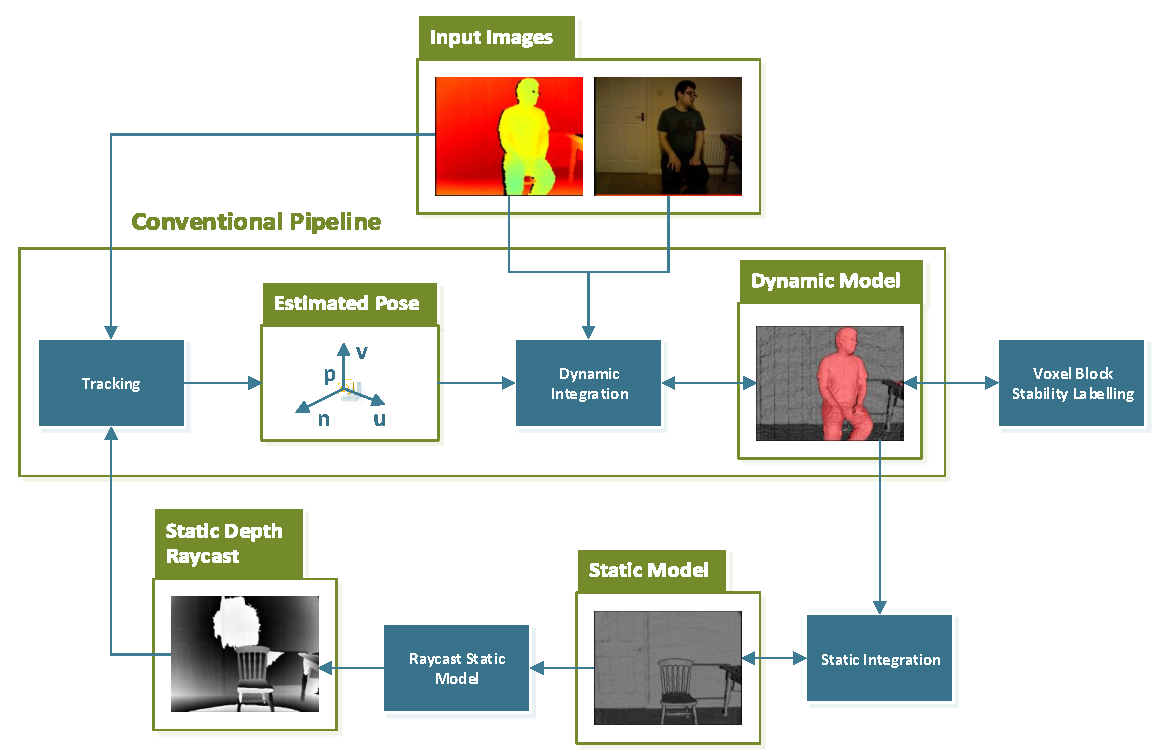
\includegraphics[width=.9\linewidth]{figures/moseg/pipeline.pdf}
  \caption[Motion Segmentation Pipeline]{The proposed motion segmentation pipeline. 
  Note the additional voxel block labelling stage with a feedback to the model 
  integration stage.}
~\label{figure:moseg_pipeline}
\end{figure}
\end{landscape}

\subsection{Stability Labelling}
~\label{sub:moseg_stability_labelling}
The purpose of the stability labelling section of the pipeline is to distinguish
between stable and unstable voxel blocks in the dynamic model, resulting in
parts of the scene that are moving being excluded from the static model. For each voxel 
block in the dynamic model, a stability value is maintained, 
representing the extent to which the instantaneous TSDF values for the voxels 
in a given voxel block (visible in the current view frustrum under the current 
pose) have remained sufficiently similar over time.

The stability value for each voxel block in the scene is initialised to nought.
At each frame, the instantaneous TSDF values for the voxels in each visible
voxel block are computed. For each voxel block, the mean absolute difference
\( \tau \), between the instantaneous and existing TSDF values is computed as
follows.
\begin{equation}
  \label{eqn:moseg_stability_value}
  \tau_{\mathcal{V}} = \Bigg[ \frac{1}{|\mathcal{V}|} \sum_{v \in \mathcal{V}}
  \bigg|\bm{\Phi}^{d}(v) - \text{min}\bigg(1, \frac{\eta}{\mu}\bigg)\bigg| \Bigg]
\end{equation}
The stability label \( l_{\mathcal{V}} \in \{\text{stable}, \text{unstable}\} \) for
a given voxel block \(\mathcal{V}\) is determined by thresholding on \( \xi \) 
(empirically set to \(0.3m\)) as follows.
\begin{equation}
  \label{eqn:moseg_stability_labelling}
  l_{\mathcal{V}} =
  \begin{cases}
    \text{stable} & \textbf{if} \mkern4mu \tau \leq \xi \\
    \text{unstable} & \textbf{if} \mkern4mu \tau > \xi
  \end{cases}
\end{equation}
If the label \(l_{\mathcal{V}}\) is ``stable'', the implication is that the voxel
block contains few disparities between the current scene and the stored model.
In this case, it's stability value is incremented. If however
\(l_{\mathcal{V}}\) has the label ``unstable'', the implication is that the
contents of the voxel block are changing, so it's stability value is reset to
nought, as follows.
\begin{equation}
  \label{eqn:moseg_stability_update}
  \tau_{\mathcal{V}} =
  \begin{cases}
    \tau_{\mathcal{V}} + 1 & \textbf{if} \mkern4mu l_{\mathcal{V}} =
    \text{stable}\\
    0 & \textbf{if} \mkern4mu l_{\mathcal{V}} = \text{unstable}
  \end{cases}
\end{equation}

Voxel blocks that are observed to be stable over a sufficiently long period of
time (empirically set to \(40\) frames) will be integrated into the static model,
as follows in Section~\ref{sub:moseg_static_to_dynamic}.

\subsection{Integration into Static Model from Dynamic Model}
~\label{sub:moseg_static_to_dynamic}
For a time step \(t\), each voxel block in the dynamic model that has assigned to
it a stable label has the entirety of it's voxel TSDF values integrated into the
static model. In a similar formulation to that given in Equation~\ref{eqn:sdf_update}
of Section~\ref{subsec:moseg_static_integration}, the update comprises 
integration of new data in to a running average.

The weight update for a given voxel \(v\) in the stable model \(\bm{\Phi}^{s}\)
with respect to a voxel (belonging to a voxel block labelled ``stable'') 
\(\bar{v}\) in the dynamic model \(\bm{\Phi}^{d}\) is given as follows.
\begin{equation}
  \label{eqn:moseg_weight_update}
  \phi^{s}_{t}(v) = \phi{(v)}^{s}_{t-1}(v) + \phi{(\bar{v})}^{d}_{t-1}(\bar{v})
\end{equation}
Similarly, the update for the TSDF values is as follows.
\begin{equation}
  \label{eqn:moseg_sdf_update}
  \bm{\Phi}^{s}_{t}(v) = \frac{1}{\phi^{s}_{t}(v)} \bigg[
  \phi^{s}_{t-1}(v) \bm{\Phi}^{s}_{t-1}(v) +
  \phi^{d}_{t-1}(\bar{v}) \bm{\Phi}^{d}_{t-1}(\bar{v})
  \bigg]
\end{equation}

\subsection{Pipeline Summary}
~\label{subsec:moseg_pipeline_summary}
With the central components of the proposed algorithm now outlined, an algorithmic 
summary may be given. As has been highlighted, the central components of the approach 
are the dual volume representation, stability labelling and inter-volume surface 
integration. The process is given in the following Algorithm.

{
  \centering
  \singlespacing{}
  \begin{minipage}{\linewidth}
    \begin{algorithm}[H]
~\label{alg:moseg}
      \caption{Motion Segmentation and Dynamic SLAM}
      \begin{algorithmic}[1]
        % $.$ used instead of \(\) due to a bug(?) in algorithmic.
        \Procedure{MoSeg Iteration}{$\bm{\Phi}_{s}, \bm{\Phi}_{d}, \bm{\Omega}, \bm{T}, t$}
          \If{\( t \neq 0 \)}
            \State{\( \mathcal{R} \gets \text{raycast}(\bm{\Phi}_{s}, \bm{\Omega}, \bm{T}) \)}
            \Comment{Section~\ref{subsec:moseg_static_rendering}}
            \State{\( \bm{T}_{t+1} \gets \text{estimatePose}(\mathcal{R}, \mathcal{D}) \)}
            \Comment{Section~\ref{subsec:moseg_static_camera_tracking}}
            \State{\( \text{updatePose}(\bm{T}_{t+1}) \)}
          \EndIf{}

          \State{\( \mathcal{D} \gets \text{unproject}(\bm{\Omega}_{d}) \)}
          \State{\( \bm{\Phi}_{d} \gets \text{integrate}(\mathcal{D}, \bm{\Phi}_{d}, \bm{T})\)}
          \Comment{Equation~\ref{eqn:sdf_update}}

          \For{\( p \in \mathcal{D} \)}
            \State{\( b \gets \text{getVoxelBlock}(p) \)}\\
            \State{\( \tau_{b} \gets \text{getStability}(b) \)}
            \Comment{Equation~\ref{eqn:moseg_stability_value}}
            \State{\( l_{b} \gets \text{getLabel}(\tau_{b}) \)}
            \Comment{Equation~\ref{eqn:moseg_stability_labelling}}
            \State{\( \text{updateStability}(b, l_{b}) \)}
            \Comment{Equation~\ref{eqn:moseg_stability_update}}\\

            \If{\( t \leq \text{initial\_frame\_count} \lor l_{b} == \text{stable} \)}
              \For{\( v \in \text{getVoxels}(b) \)}
                \State{\( \phi_{s}(v) \gets \text{getWeight}(v) \)}
                \State{\( \phi_{d}(v) \gets \text{getWeight}(v) \)}
                \State{\( \bm{\Phi}_{s}(v) \gets \text{integrate}(\bm{\Phi}_{s}(v), 
                \bm{\Phi}_{d}(v)), \phi_{s}(v), \phi_{d}(v) \)}
                \Comment{Equation~\ref{eqn:moseg_sdf_update}}
                \State{\( \text{updateStableWeight}(\phi_{s}(v), \phi_{d}(v)) \)}
                \Comment{Equation~\ref{eqn:moseg_weight_update}}
              \EndFor{}
            \EndIf{}
          \EndFor{}

          \State{\( \text{raycast}(\bm{(\Phi)}_{d}, \bm{T}) \)}
          \Comment{Visualise Dynamics}
        \EndProcedure{}
      \end{algorithmic}
    \end{algorithm}
  \end{minipage}
  \par
}
% TODO: Spacing. Gap not showing.
The presented Algorithm is trivially parallelisable with commodity GPU hardware.
The integration of points in the depth map \( \mathcal{D} \) is parallelisable 
with minimal risk of race conditions occurring. However care must be taken for edge 
cases where multiple simultaneous writes may occur at the same TSDF location. 
However, the integration of TSDF data from the dynamic model to the static model 
has no such risk and as such is trivially parallelisable.

\section{Qualitative Results}
~\label{sec:moseg_qualitative}
Empirically, the proposed motion segmentation system is capable of retaining
globally consistent tracking within the dense SLAM framework for a range of
scenarios that would prove to be problematic for other, static dense SLAM
systems. The experiments performed demonstrate a robustness	to dynamics in
various scenes, both in terms of tracking and noise artefacts in the static
model. In addition, the system is robust to the addition and removal of scene
components and is robust to short term occlusions, such as a person walking in
front of the camera. An example of a person moving in to the the view frustrum
and sitting on a Setee is given in Figure~\ref{figure:moseg_qualitative_setee}.

\begin{figure}[!htbp]
  \centering
  \begin{tabular}{ccc}
    % TODO: Middle picture is smaller.
    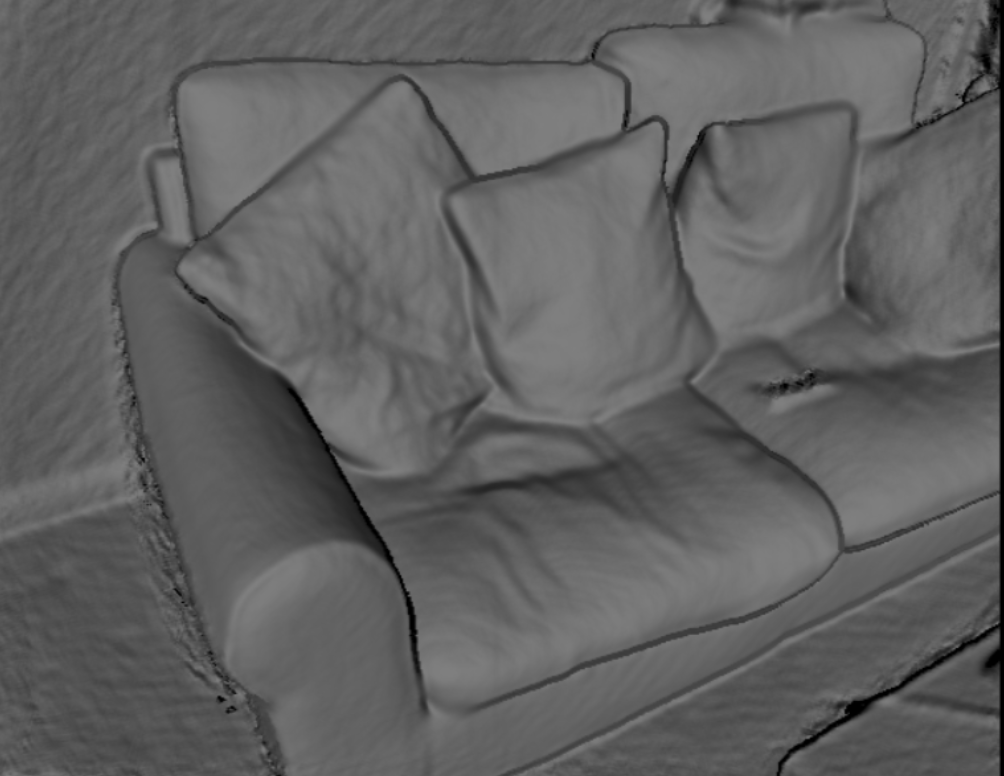
\includegraphics[width=.3\linewidth]{figures/moseg/original_sitting.png} &
    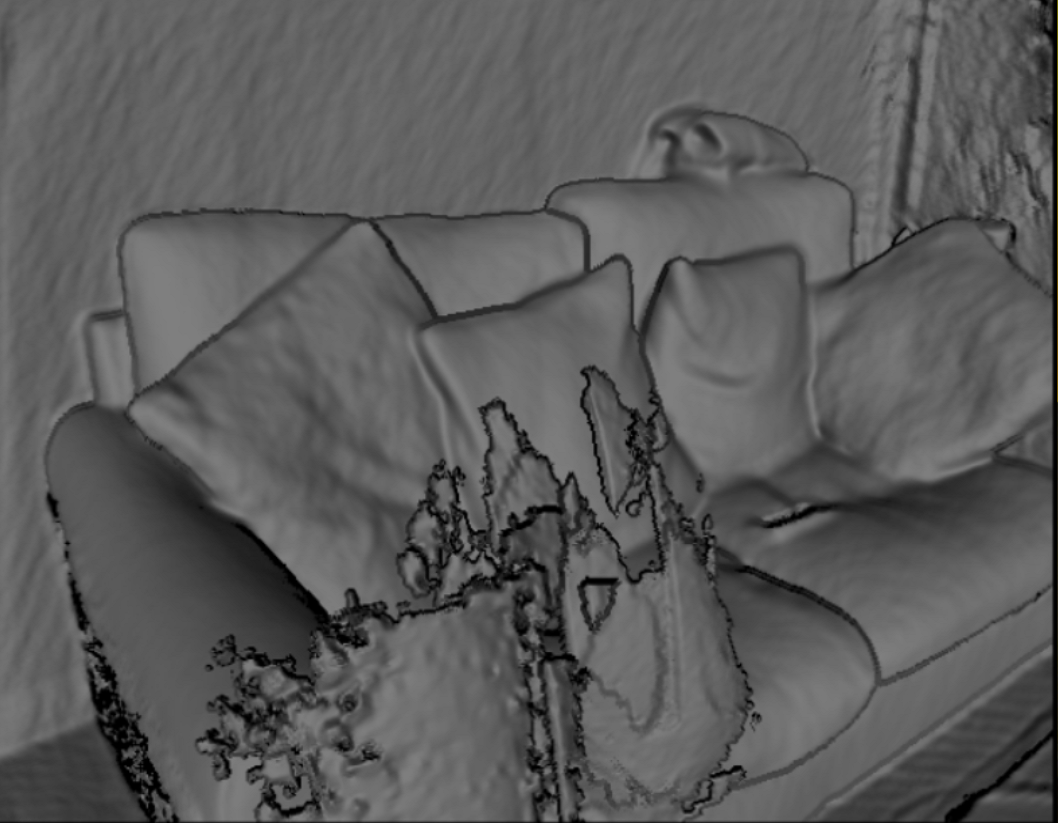
\includegraphics[width=.3\linewidth]{figures/moseg/infinitam_sitting.png} &
    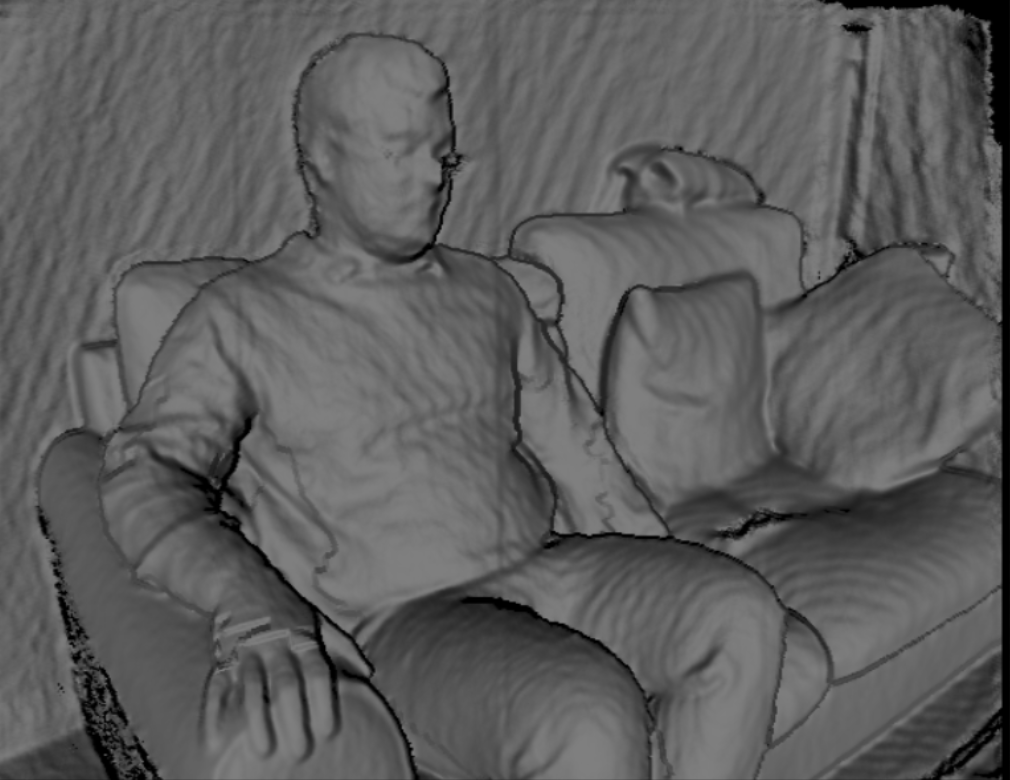
\includegraphics[width=.3\linewidth]{figures/moseg/moseg_sitting.png}\\
    (a) & (b) & (c)
  \end{tabular}
  \caption[Motion Segmentation Qualitative Results I]
  {
    \begin{tabular}[t]{@{}l@{}}
      A qualitative comparison between the proposed system and InfiniTAM~\cite{Prisacariu2014}.\\
      (a) A static scene containing a Setee is reconstructed.\\
      (b) When a person enters the scene using standard InfiniTAM, the tracking
      fails,\\ leading to a corrupted scene model.\\
      (c) Using the proposed system, tracking is maintained and the person is\\
      integrated successfully into the scene.
    \end{tabular}
  }
~\label{figure:moseg_qualitative_setee}
\end{figure}

In addition to the ability to reconstruct a moving object that becomes static in
the scene as shown in Figure~\ref{figure:moseg_qualitative_setee}, the proposed
system is also capable of segmenting dynamic objects in a scene that are
undergoing nonrigid motion. Whilst these objects are segmented and labelled as
``dynamic'' they are not used for camera pose estimation. An example of this
behaviour may be observed in Figure~\ref{figure:moseg_qualitative_chair}.

\begin{figure}[!htbp]
  \centering
  \begin{tabular}{cc}
    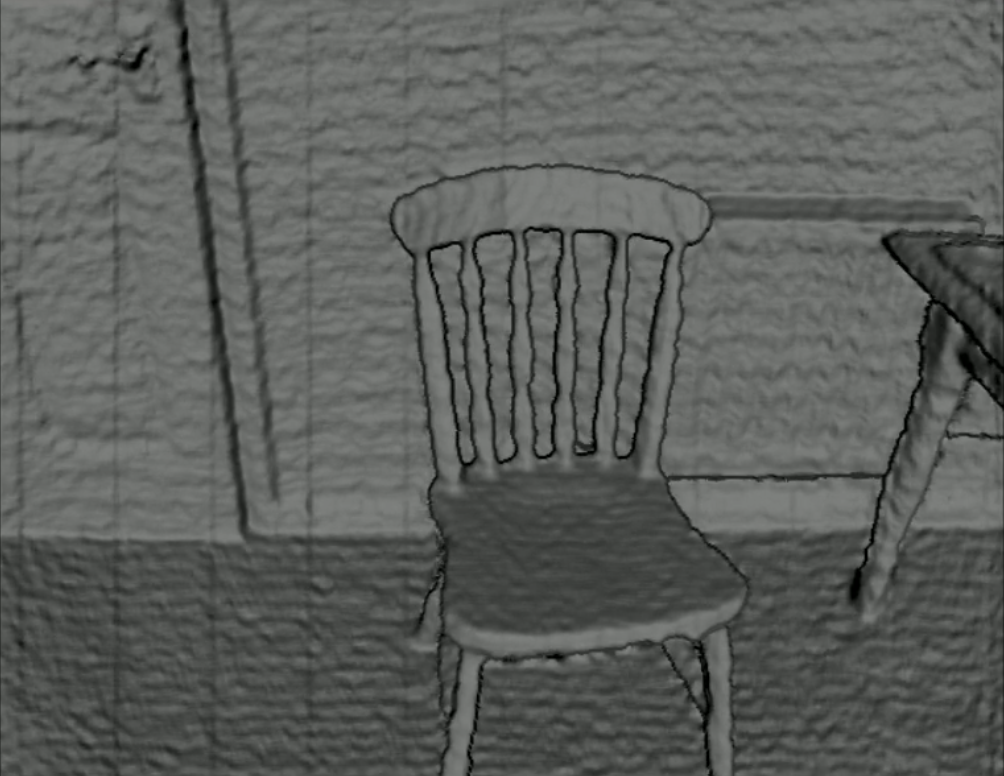
\includegraphics[width=.4\linewidth]{figures/moseg/chair0.png} &
    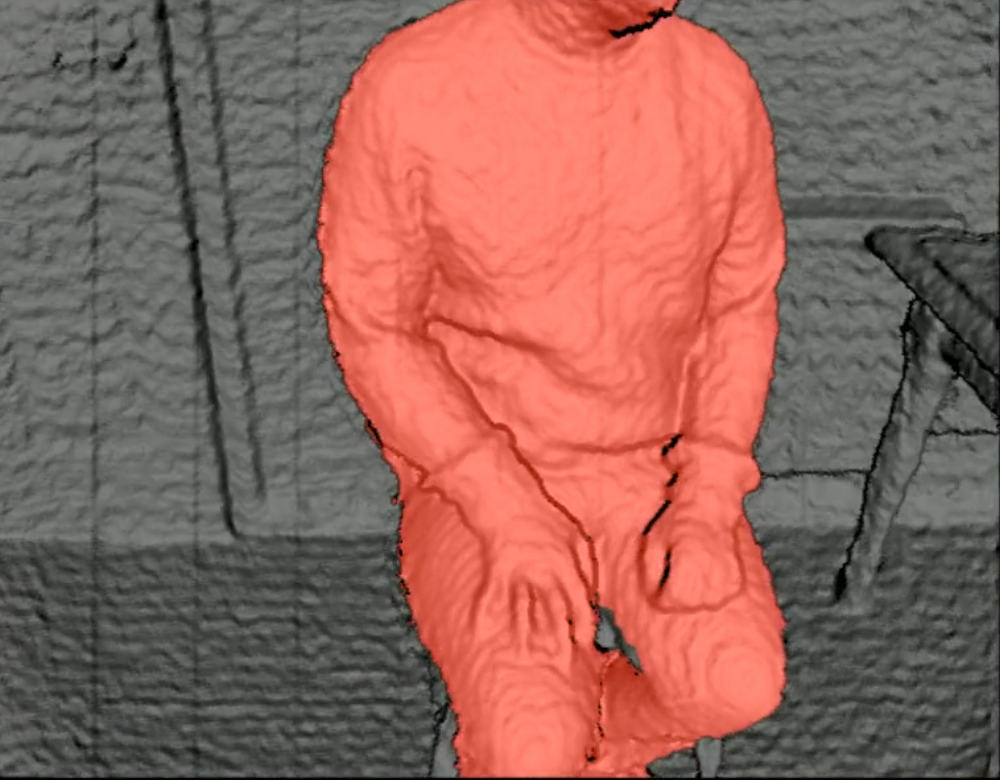
\includegraphics[width=.4\linewidth]{figures/moseg/chair1.png} \\
    (a) & (b) \\
    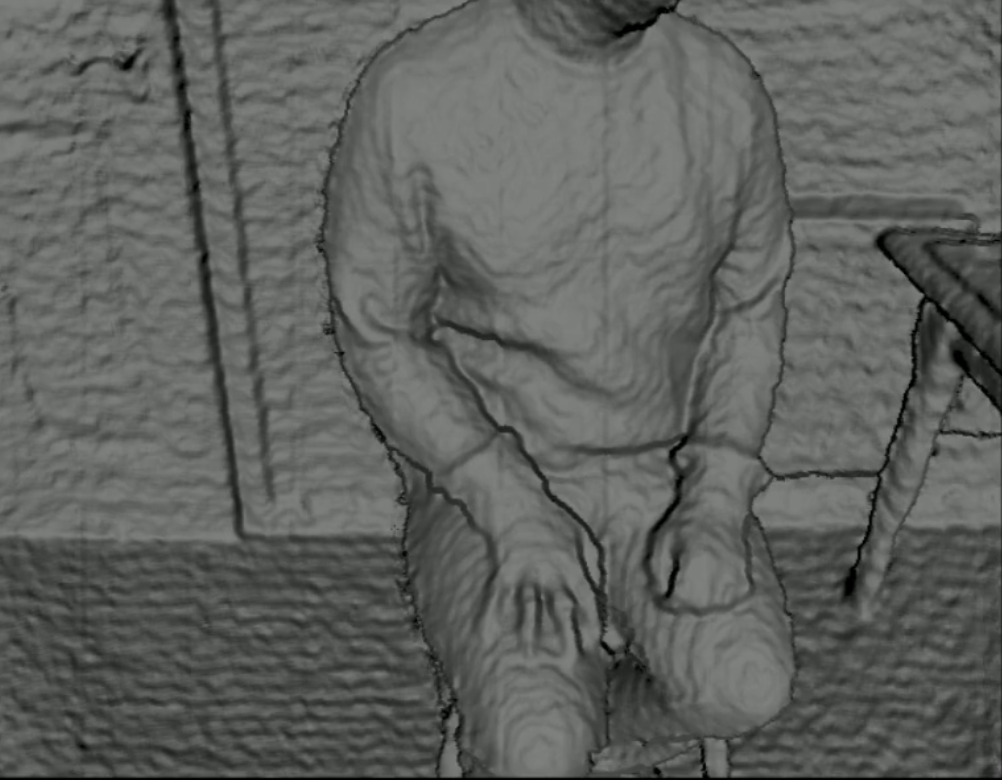
\includegraphics[width=.4\linewidth]{figures/moseg/chair2.png} &
    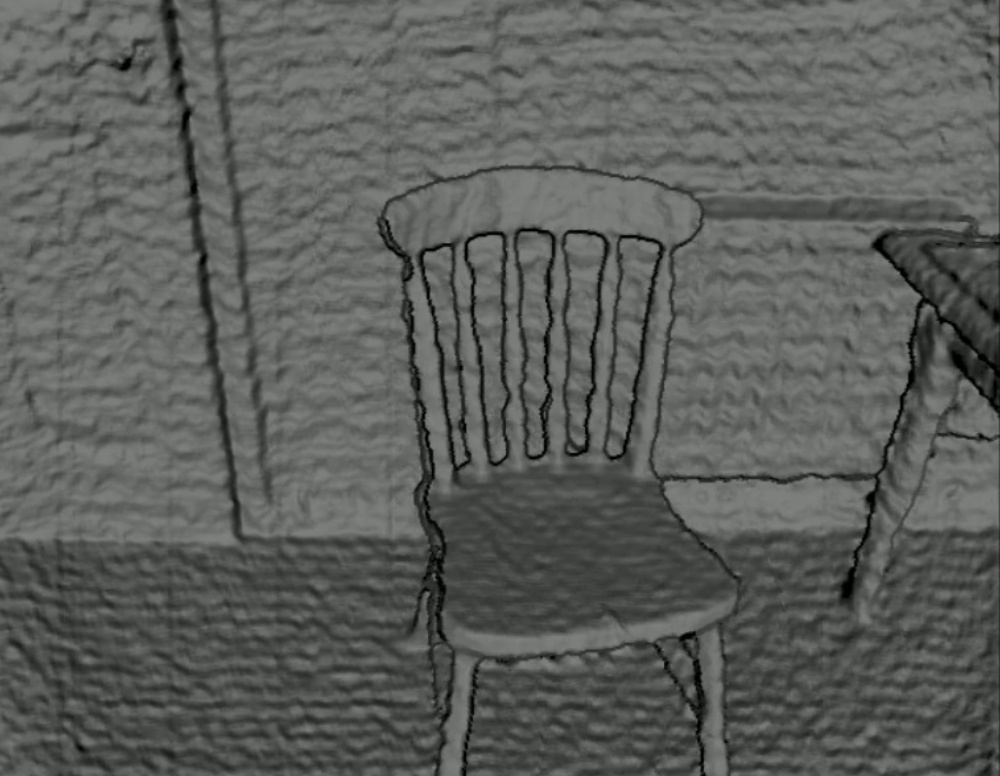
\includegraphics[width=.4\linewidth]{figures/moseg/chair3.png} \\
    (c) & (d)
  \end{tabular}
  \caption[Motion Segmentation Qualitative Results II]
  {
    \begin{tabular}[t]{@{}l@{}}
      A qualitative example of the proposed systems ability to segment\\
      dynamic scene components.\\
      (a) A static scene containing a Chair is reconstructed.\\
      (b) A person enters the scene, is marked as \textit{dynamic} and sits down.\\
      (c) After gaining a sufficient confidence score, the person is labelled\\
      \textit{static} and is integrated in to the static model.\\
      (d) The person gets up from the Chair and leaves the scene.\\ The original
      reconstruction of the Chair from (a) is in tact.
    \end{tabular}
  }
~\label{figure:moseg_qualitative_chair}
\end{figure}

\section{Quantitative Results}
~\label{sec:moseg_quantitative}
In this section, a quantitative evaluation of the system's efficacy in terms of
and camera tracking ability is provided.

For the quantitative analysis, the system has been evaluated on the dynamic
objects subset of the TUM\footnotemark RGBD dataset~\cite{Sturm2012} with respect to
trajectory quality. The scenes provided in the dataset contain a range of
dynamic components ranging from arm movement to people walking around, occluding
parts of the scene. Comparison is drawn against the standard InfiniTAM framework
on which the proposed system is based, using standard, static InfiniTAM as a
baseline.
~\footnotetext{Technical University of Munich, RGB-D SLAM Dataset and Benchmark.\\
\url{https://vision.in.tum.de/data/datasets/rgbd-dataset}}

\begin{table}[!htbp]
\begin{center}
  \begin{tabular}{l c c}
    \emph{TUM Standard Sequence Name} & \emph{MoSeg} ATE & \emph{Baseline} ATE \\
    \midrule
    \textsf{fr2-desk-with-person} & \textbf{0.158 \std{0.091}} & 0.297 \std{0.193}\\
    \textsf{fr3-sitting-static} & 0.014 \std{0.008} & \textbf{0.012 \std{0.007}}\\
    \textsf{fr3-sitting-xyz} & 0.064 \std{0.031} & \textbf{0.053 \std{0.029}}\\
    \textsf{fr3-sitting-halfsphere} & 0.142 \std{0.063} & \textbf{0.115 \std{0.049}}\\
    \textsf{fr3-sitting-rpy} & \textbf{0.056 \std{0.033}} & 0.081 \std{0.051}\\
    \textsf{fr3-walking-static} & \textbf{0.294 \std{0.153}} & 0.999 \std{0.178}\\
    \textsf{fr3-walking-xyz} & \textbf{0.385 \std{0.271}} & 0.544 \std{0.343}\\
    \textsf{fr3-walking-halfsphere} & \textbf{0.539 \std{0.360}} & 0.762 \std{0.367}\\
    \textsf{fr3-walking-rpy} & \textbf{0.662 \std{0.335}} & 0.843 \std{0.365}\\
  \end{tabular}
\end{center}
\caption[Motion Segmentation ATE]
{The Absolute Trajectory Error (ATE) results (in metres, lower is better) 
achieved by the proposed approach in comparison to the baseline InfiniTAM
~\cite{Prisacariu2014} framework on a variety of the standard sequences from
  the TUM RGBD dataset~\cite{Sturm2012}. Results are in the format mean
  \( \pm \) standard deviation. The better result (by mean) on each sequence is
  highlighted in bold.}
~\label{table:moseg_ate}
\end{table}

Given in Table~\ref{table:moseg_ate} is the Absolute Trajectory Error (ATE) measures
for each of the TUM Dynamic Scenes. The ATE utilises the method of Horn~\cite{Horn1987} to 
solve for the error incurred by mapping the trajectory of the proposed system on to the ground 
truth trajectory of the TUM sequence, for a given TUM Dynamic Objects sequence. The results of 
Table~\ref{table:moseg_ate} are visualised in Figure~\ref{figure:moseg_ate}.

\begin{figure}[!htbp]
  \centering
  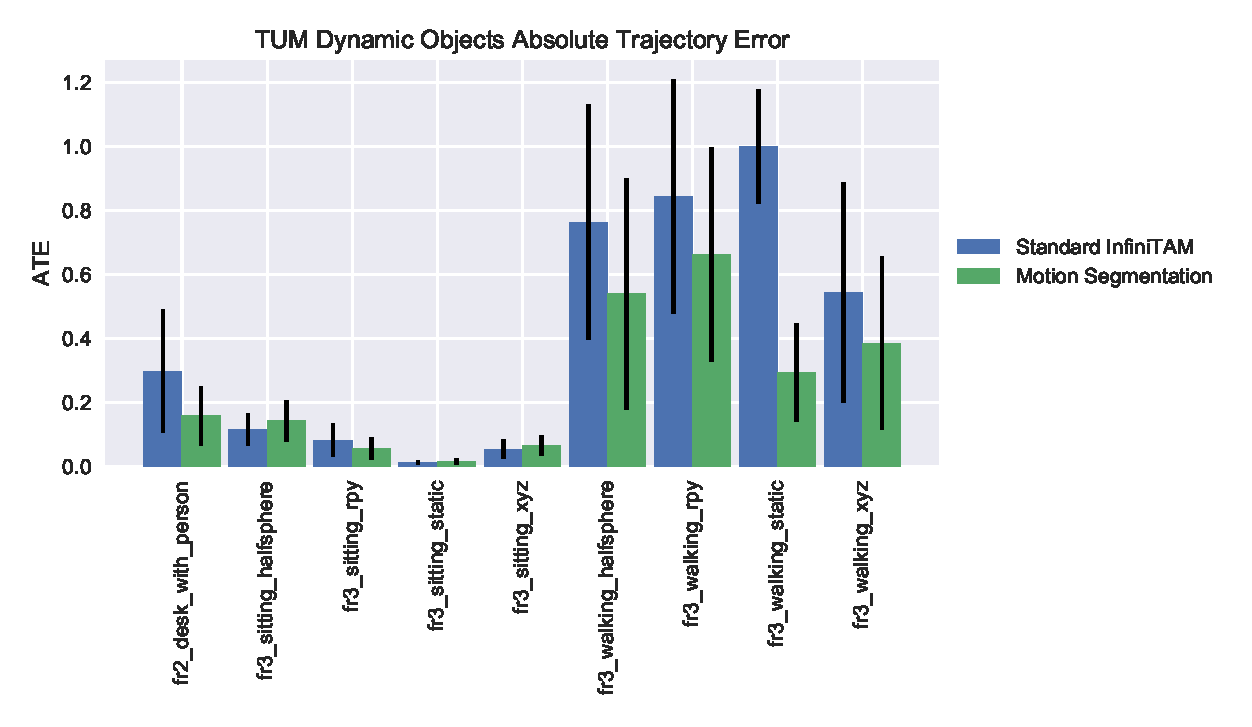
\includegraphics[width=\linewidth]{figures/moseg/ate.eps}
  \caption[Motion Segmentation ATE]
  {Absolute Trajectory Error (ATE) for the TUM Dynamic Scenes dataset.}
~\label{figure:moseg_ate}
\end{figure}

In addition to evaluating quantitatively in terms of Absolute Trajectory Error,
additional results are provided in terms of Relative Trajectory Error (RTE)
~\cite{Sturm2012}. RTE measures the relative pose error over a fixed time
interval, with the final score being the Root Mean Squared Error (RMSE) over all 
time windows. RTE results are provided in Table~\ref{table:moseg_rte} and visualised 
in Figure~\ref{figure:moseg_rte}.

\begin{table}[!htbp]
\begin{center}
  \begin{tabular}{l c c}
    \emph{TUM Standard Sequence Name} & \emph{MoSeg} RTE & \emph{Baseline} RTE \\
    \midrule
    \textsf{fr2-desk-with-person} & \textbf{0.023 \std{0.030}} & 0.026 \std{0.037}\\
    \textsf{fr3-sitting-static} & 0.010 \std{0.008} & \textbf{0.010 \std{0.008}}\\
    \textsf{fr3-sitting-xyz} & 0.028 \std{0.017} & \textbf{0.028 \std{0.017}}\\
    \textsf{fr3-sitting-halfsphere} & \textbf{0.031 \std{0.033}} & 0.032 \std{0.029}\\
    \textsf{fr3-sitting-rpy} & 0.073 \std{0.061} & \textbf{0.067 \std{0.065}}\\
    \textsf{fr3-walking-static} & \textbf{0.082 \std{0.140}} & 0.163 \std{0.308}\\
    \textsf{fr3-walking-xyz} & 0.410 \std{0.262} & \textbf{0.300 \std{0.252}}\\
    \textsf{fr3-walking-halfsphere} & \textbf{0.245 \std{0.320}} & 0.305 \std{0.374}\\
    \textsf{fr3-walking-rpy} & 0.482 \std{0.456} & \textbf{0.406 \std{0.364}}\\
  \end{tabular}
\end{center}
\caption[Motion Segmentation RTE]
{The Relative Trajectory Error (RTE) results (in metres, lower is better) 
achieved by the proposed approach in comparison to the baseline InfiniTAM
~\cite{Prisacariu2014} framework on a variety of the standard sequences from
the TUM RGBD dataset~\cite{Sturm2012}. Results are in the format mean
\( \pm \) standard deviation. The better result (by mean) on each sequence is
highlighted in bold.}
~\label{table:moseg_rte}
\end{table}

\begin{figure}[!htbp]
  \centering
  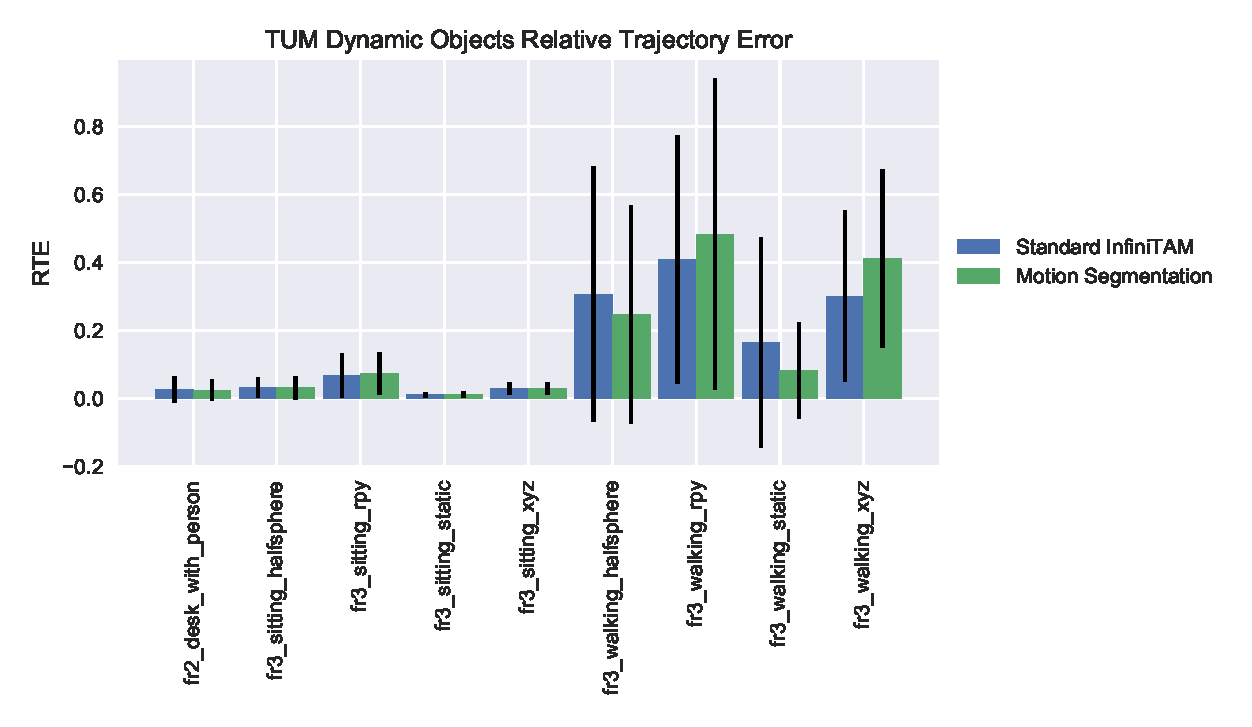
\includegraphics[width=\linewidth]{figures/moseg/rte.eps}
  \caption[Motion Segmentation RTE]
  {Relative Trajectory Error (RTE) for the TUM Dynamic Scenes dataset.}
~\label{figure:moseg_rte}
\end{figure}

\section{Performance Evaluation}
~\label{sec:moseg_performance}
As outlined in the research objectives of Section~\ref{sec:intro_aims_structure}, the proposed 
dynamic SLAM pipeline is required to run in real-time if it is to be suitable for use at scale. 
The basic dense SLAM pipeline of \textit{Prisacariu et al}~\cite{Prisacariu2014} is a highly 
optimised implementation of the Voxel Hashing approach of \textit{Nei{\ss}ner et al}~\cite{NieBner2013}, 
achieving very high framerates on consumer computing equipment. For the purpose of evaluating the 
performance of the modified pipeline outlined in this work, a direct comparison is drawn to 
\textit{InfiniTAM}, the implementation of \textit{Prisacariu et al}~\cite{Prisacariu2014}.
\begin{figure}[!htbp]
  \centering
  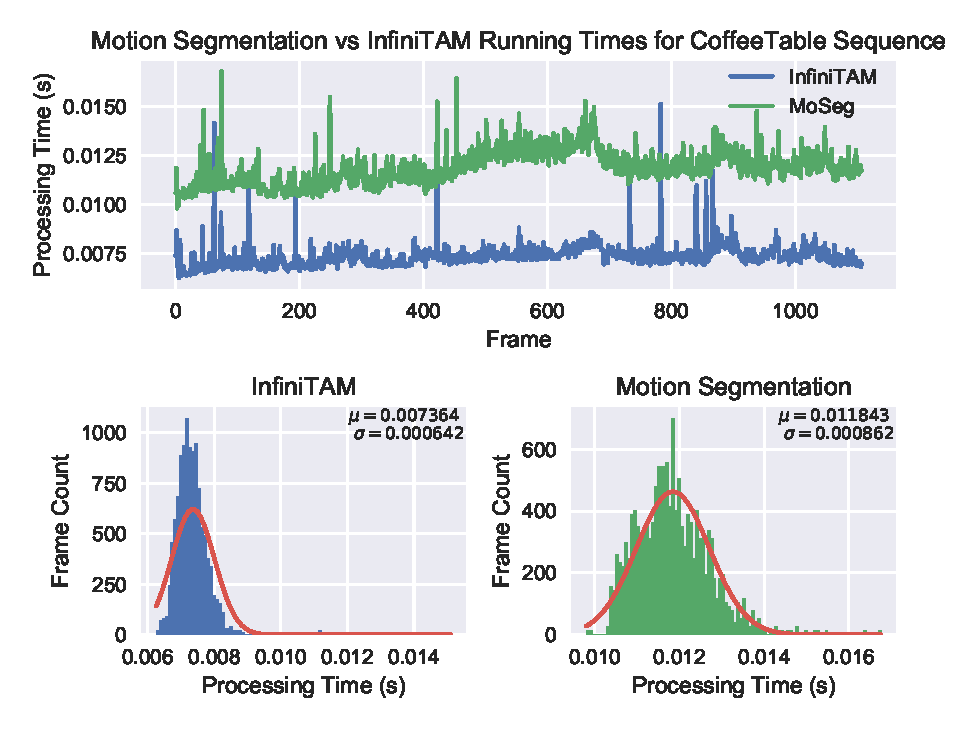
\includegraphics[width=\linewidth]{figures/moseg/timings_coffee.eps}
  \caption[Motion Segmentation Performance on CoffeeTable Sequence]
  {Performance of the proposed approach versus the standard dense SLAM pipeline of 
  \textit{Prisacariu et al}~\cite{Prisacariu2014}.}
~\label{figure:moseg_timing_coffee}
\end{figure}

It can be seen from Figure~\ref{figure:moseg_timing_coffee} that the motion segmentation and 
dynamic SLAM system proposed in this work is capable of operating at above real time performance. The 
sequence from which the performance statistics of Figure~\ref{figure:moseg_timing_coffee} are derived 
consists of 1108 frames in which dynamics are prevalent throughout. It can be seen that although the 
cost of the proposed system is higher than that of the standard SLAM pipeline, performance is still 
better than real-time. It should be noted however that the mean processing time for a given frame 
is 0.011843 seconds, the standard deviation over the sequence is 0.000862 seconds. Such varying per 
frame times are due to the varying degree of observed dynamic scene components. However, the proposed 
approach performs at \(\approx 84Hz\) versus the standard pipeline's performance of \(\approx 136Hz\), 
indicating a non detrimental performance deficit.

\section{Application to Semantic Scene Understanding}
~\label{sec:moseg_semantic}
The dynamic scene handling approach described in Section~\ref{sec:moseg_dynamic_fusion}
can be used to prevent moving objects from being integrated into the static
scene model. However, for many applications (e.g.\ mobile robotics), there is an
additional need to understand what objects are present in the scene and where
they are, as outlined in Section~\ref{sec:intro_scene_recon}. In this section, it is 
therefore shown that classifiers may be trained for the moving objects and used to recognise 
new instances of those objects as they enter the scene.

The voxel blocks in the dynamic model that were identified as ``unstable''
provide a natural representation of the dynamic parts of the scene. Where
multiple dynamic objects are present, they can be separated by finding the
connected components of these voxel blocks. For each object, a one-class Support
Vector Machine (SVM)~\cite{Singer07} with a polynomial kernel is trained and used 
to recognise new instances of the object class.

Upon seeing a new object, the system first tries to classify the object into a category
that has already been seen, by predicting the objects class with all of the existing single class 
SVMs. If this fails, the system generates a label for the object and trains a new SVM for it's 
class. 

To make the training examples for the detected object, points are uniformly sampled from the object's
isosurface and Fast Point Feature Histogram (FPFH) descriptors~\cite{Rusu2009} are computed
at these points. FPFH descriptors are geometric features that provide a
per-point statistic of the curvature within some neighbourhood of the point
(empirically, a \(2.5cm\) radius around the point is used). Figure~\ref{figure:moseg_recognition} 
shows an example of this training and prediction process for dynamic objects.

\begin{figure}[!htbp]
  \centering
  \begin{tabular}{ccc}
    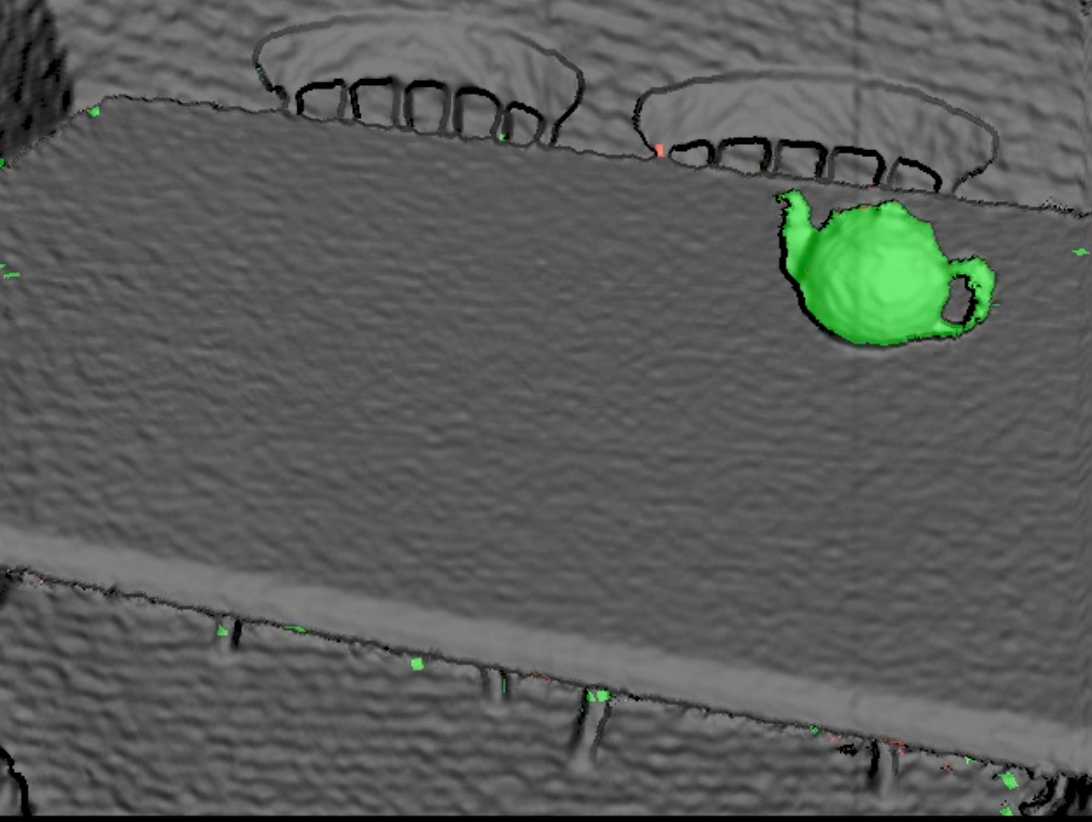
\includegraphics[width=.3\linewidth]{figures/moseg/objects1.png} &
    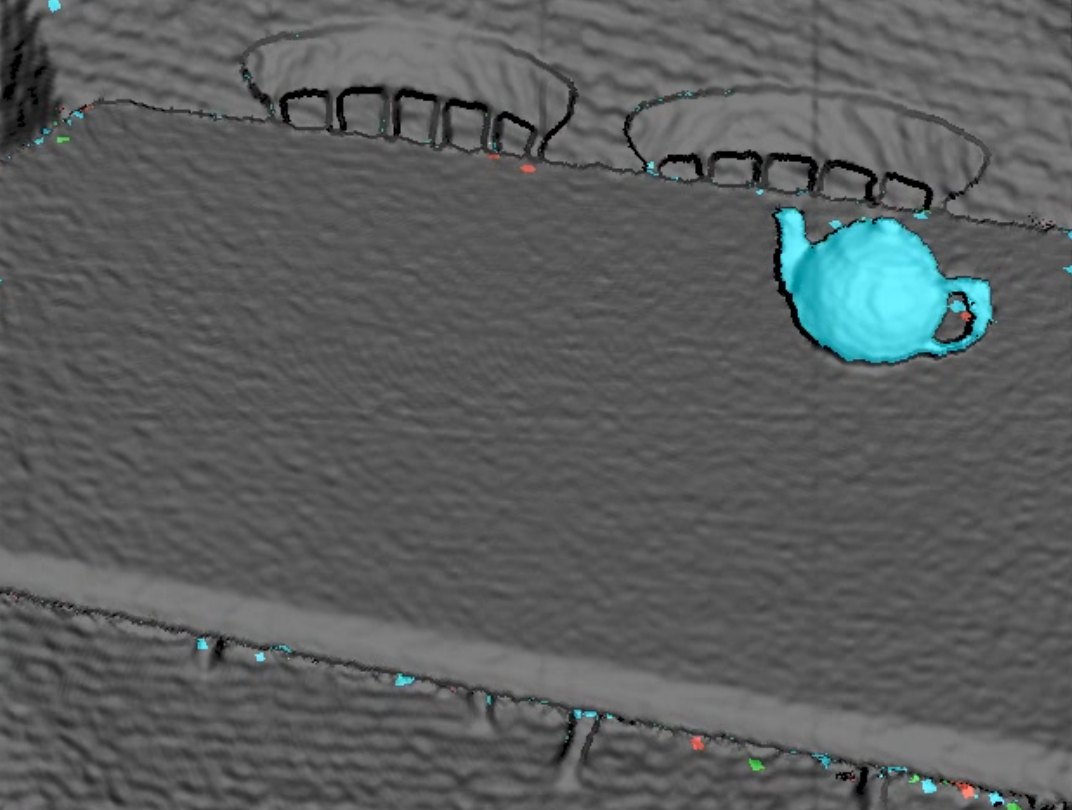
\includegraphics[width=.3\linewidth]{figures/moseg/objects2.png} &
    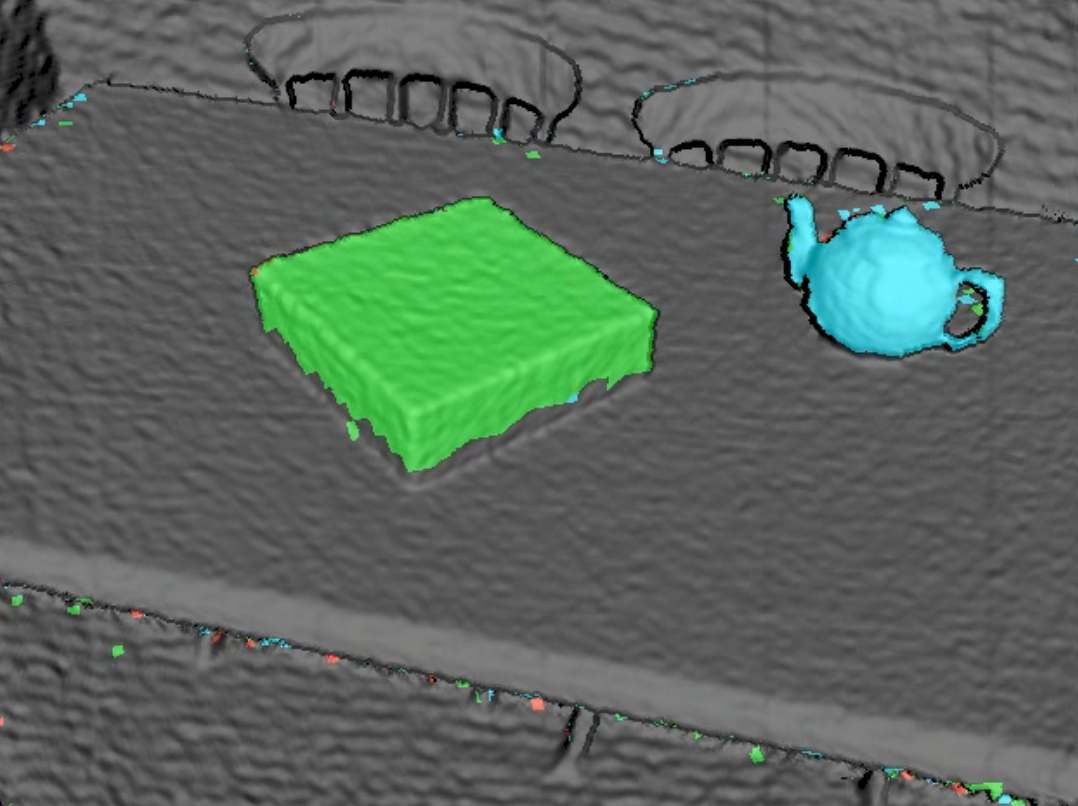
\includegraphics[width=.3\linewidth]{figures/moseg/objects3.png} \\ 
    (a) & (b) & (c) \\
    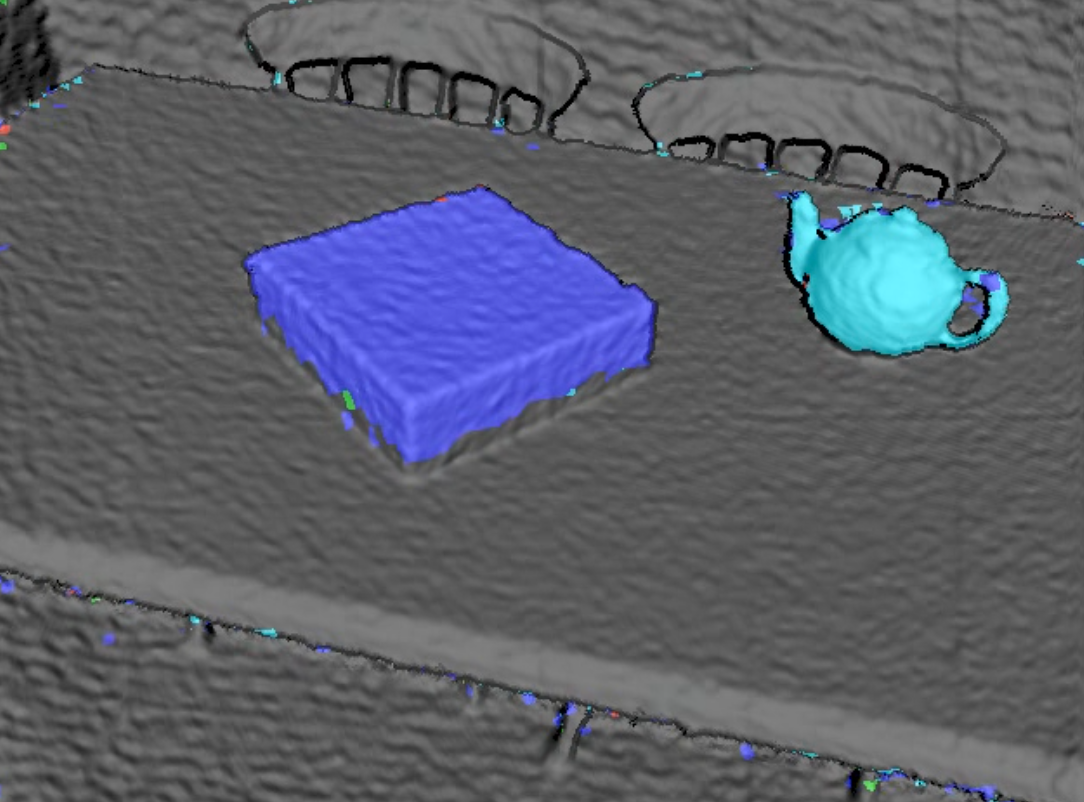
\includegraphics[width=.3\linewidth]{figures/moseg/objects4.png} &
    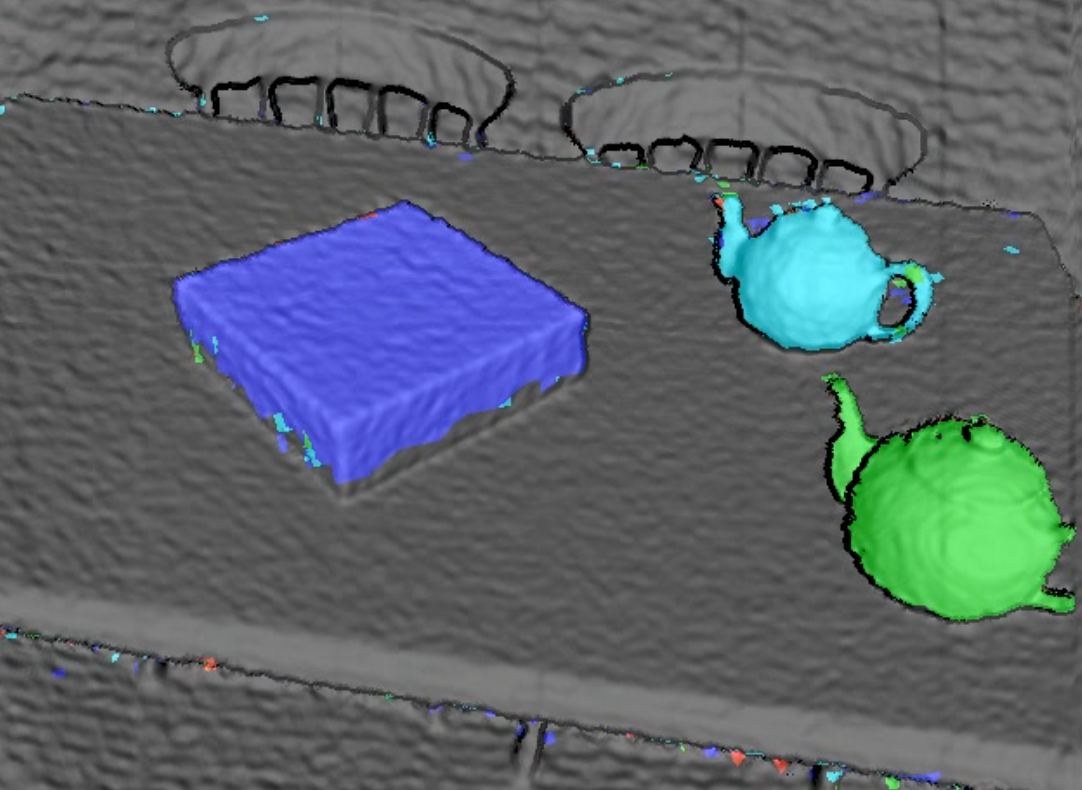
\includegraphics[width=.3\linewidth]{figures/moseg/objects5.png} &
    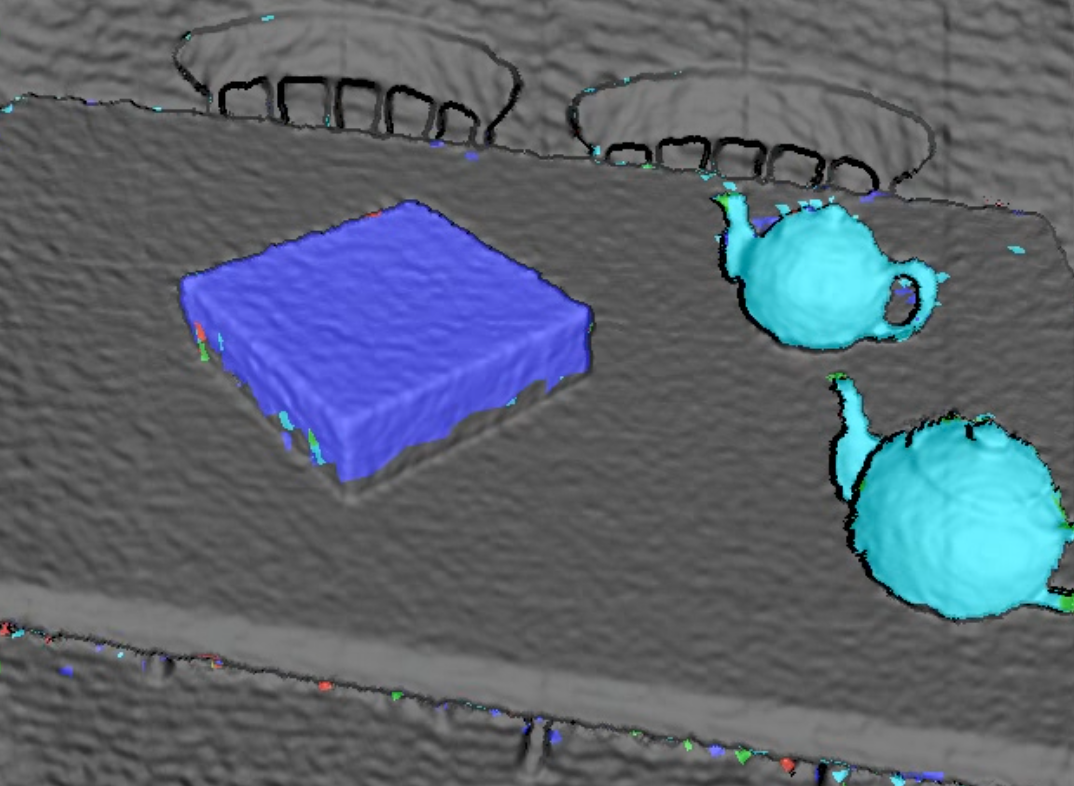
\includegraphics[width=.3\linewidth]{figures/moseg/objects6.png} \\ 
    (d) & (e) & (f) \\
  \end{tabular}
  \caption[Motion Segmentation Object Recognition]
  {
    \begin{tabular}[t]{@{}l@{}}
      An example of the training and prediction process for dynamic objects:\\
      (a) A teapot is placed in the scene.\\
      (b) The teapot is recognised as a new object and an SVM is trained for it.\\
      (c) A box is placed in the scene.\\ 
      (d) The box is recognised as being distinct from the teapot, so a separate \\SVM is trained.\\
      (e) Another teapot is placed in the scene.\\
      (f) The new teapot is recognised, and is labelled accordingly.
    \end{tabular}
  }
~\label{figure:moseg_recognition}
\end{figure}

\section{Summary}
~\label{sec:moseg_discussion}
As outlined in Sections~\ref{sec:moseg_qualitative} and~\ref{sec:moseg_quantitative}, the 
proposed approach provides an improvement on the quality of camera pose estimation when 
performing dense reconstruction in scenes that have dynamic components, versus the 
standard \textit{KinectFusion}~\cite{Newcombe2011} like pipeline as implemented by 
\textit{Prisacariu et al}~\cite{Prisacariu2014}; a research objective that was outlined in 
Section~\ref{sec:intro_aims_structure}.

Additionally, it is evident that the proposed approach is capable of segmenting dynamic 
components (such as people moving in an articulated fashion) that are visible in the camera's 
view frustrum, from those that are static (such as furniture in the scene). This segmentation 
also demonstrates a novel way of obtaining 3D geometry information to perform rudimentary scene 
understanding. Additionally, the resultant reconstructions of the proposed approach are 
qualitatively comparable to the comparison static dense SLAM system. Both of these results 
relate again to the research objectives of Section~\ref{sec:intro_aims_structure}.

The novel dual volumetric representation approach taken in this work of maintaining both a 
\textit{static} and a \textit{dynamic} scene, utilising only the former for camera pose 
estimation provides a simple and robust system for dense 3D reconstruction in environments 
that would otherwise be troublesome. Contrary to existing approaches outlined in Section 
~\ref{sec:lit_review_dynamic}, the presented system has scope for use in large-scale 
reconstruction scenarios, due to it's leverage of efficient, hashed volumetric data structures. 
In addition, by utilising such data structures, the proposed system is performant to the 
level of highly optimised~\cite{Prisacariu2014} \textit{KinectFusion}~\cite{Newcombe2011} 
implementations, demonstrating feasibility for application to problems that require 
real time performance.

With the contributions outlined in this work, the proposed approach provides a platform 
for further research into problems such as live semantic scene understanding and dense scene 
flow. The proposed approach has the potential to be further developed in to a fully dynamic, 
semantic scene understanding and reconstruction system for use in robotics, VR and AR applications 
as outlined in Section~\ref{sec:intro_scene_recon}. Though as previously outlined, the contributions 
of this chapter allow for the extraction of 3D geometry data for machine learning purposes, it is 
reliant on the detection of motion. As such, the topic of Chapter~\ref{chap:probobj} is 3D object 
reconstruction.